\documentclass[]{report}   % list options between brackets
\usepackage{graphicx,url,placeins,algorithm,algorithmic,lipsum,amssymb,amsmath,subfigure,float}
\usepackage[hidelinks]{hyperref}
\graphicspath{{figures/}}

\begin{document}

\title{TN1008\\ Project Report}   % type title between braces
\author{
  Viktor Nilsson, vikni067@student.liu.se 
  \\Axel Kinner,
  \\Johannes Deligiannis, johde901@student.liu.se
  \\Johan Beck-Norén, johbe559@student.liu.se
  \\Andreas Valter, andva287@student.liu.se
	}
        \date{\today}    % type date between braces
        \maketitle
        
\setcounter{page}{2}

\begin{abstract}

\end{abstract}

\begingroup
\let\clearpage\relax % Removes blankpage before include
\chapter{Introduction}
\section{What is fire?}
By fully understanding the process behind fires one can easier simulate and render the phenomena. Fires are usually created by a chemical reaction between oxygen and fuel. As the amount of oxygen is reduced the flame becomes less clean resulting in appearing smoke. 

The chemical reaction is most commonly producing carbon dioxide, heat and light. The actual flame that we can see is then the combined outcome of all three products. Depending on the temperature of the flame; it appears differently when observed by the human eye. This is due to the Black-body radiation emitted from the fuel, gas and soot particles.

\section{Different ways to simulate fire}
The most correct state of the art approach for producing flames is to track the burnt fuel and the unburnt fuel as two separate fluids. By tracking the temperature of the two; the simulation ignites the unburnt fuel when reaching a specific temperature and reduces the burnt fuel over the time. To create a lasting flame one has to add unburnt fuel over the simulation time. This assumes that the system is surrounded by an oxidizer (e.g air).

Other approaches includes to create the flames procedurally, without using any fluid system. This is ofcourse much easier and faster to implement. There is also some fluid approaches that track one fluid; the flame surface (density) instead of the temperature.

\section{General fluid simulation background}
Fluid simulation has been around before we even started to use computers. The first mathematical approaches were presented around 1950. Incompressible and free-surface fluids were first seen around 1996(ref FosterMetaxas). Before this the fluids were computed as non physically-based and in 2D.

Since the Navier-Stokes equations are still yet to be solved many different approaches and methods for fluid simulation exists.

\section{Previous implementations of fire}
The most notable previous report; and the one this report followed is Physically Based Modeling and Animation of Fire(ref Nguyen02). It approaches the problem as described earlier with two seperated fluids and combines them with the help of a ghost fluid in between them. There exist many new improved methods based on Nguyen02 such as Wrinkled Flames and Cellular Patterns(ref), which introduces the characteristic surface a flame often have.

\chapter{Background}
\section{Physically Based Model}
Visually, one can define two distinct components of fire or flames; the inner blue core and the hot gaseous products. In this report we follow the technique used in REF TILL RAPPORT for tracking the border between the blue core and the hot gaseous products with an implicit surface (level set). The inside of the surface is defined as the gaseous fuel which has yet to be ignited, and the outside of the surface is defined as the ignited hot gaseous products. The black-body radiation emitted by the ignited fuel (hot gaseous products) are what we typically see as the orange or yellow coloured component of fire. We also track the temperature in order to enable us to discern between the blue core and hot gaseous products, and to be able to render the simulation with visual accuracy. The gaseous fuel is injected at its ignition temperature, and as fuel crosses over our implicit surface (igniting) its temperature cools until the black-body radiation is indistinguishable from the surrounding air.
\subsection{Blue Core}
As stated earlier, we separate the gaseous fuel from the ignited fuel by an implicit surface. This implicit surface moves at a velocity of the unreacted fuel velocity plus a flame speed \emph{S}. \emph{S} dictates at what rate the fuel is burning (moving over the implicit surface), and will produce different kinds of flames for different values for \emph{S}. A small value for \emph{S} will result in a blue core with greater surface area, and vice versa for a larger value for \emph{S}.
\subsection{Hot Gaseous Products}
The blackbody radiation emitted from the hot gaseous products is the part of the flame we often consider being yellow or orange. To be able to represent these colours when rendering the simulation we track the temperature across our grids. Another important aspect of the simulation is the expansion that takes place as the fuel passes over our implicit surface and ignites. A simplified explanation of what happens is an almost instantaneous expansion of the fuel as it ignites, causing a change in the fuel trajectory as it does so. We model this in the same fashion as in REF TILL RAPPORT HÄR, by using a density ratio between the density for the fuel and the hot gaseous product respectively. Since we assume that mass and momentum are preserved, we use the following equations from REF TILL RAPPORT HÄR to couple the flow equations across the implicit surface.
\begin{equation}
\rho_h(V_h-D) = \rho_f(V_f-D),
\end{equation}
\begin{equation}
\rho_h(V_h-D)^2+p_h = \rho_f(V_f-D)^2+p_f
\end{equation}
In these equations $V_h$ and $V_f$ are the velocities in the normal direction for the hot gaseous products and the fuel respectively, $D = V_f+S$ is the implicit surface's speed in the normal direction, and $p_h$ and $p_f$ are the pressures for the hot gaseous products and the fuel. Note that this rapid expansion causes discontinuities in both the density and the velocities in the area of the blue core border (the implicit surface). We must therefore be careful when taking derivatives in that region, which brings us to the next section.
\subsection{Two-phase Flow and Ghost Fluid Method}
We model the fuel and the hot gaseous products by two separate sets of incompressible flow equations, namely Navier-Stokes equations. The problem with discontinuities along the blue core surface described in the previous section can be solved by extrapolating values for each section (fuel and hot gaseous products) by the Ghost Fluid Method REF TILL GHOST-RAPPORT HÄR. If we  for example are taking the derivative for the unignited fuel in the vicinity of the blue core, we will extrapolate fuel velocity values for cells adjacent to, but outside of, the blue core. These extrapolated values can then be used when taking derivatives and we do not have to worry about the discontinuities described earlier. Vice versa for ignited fuel in the vicinity of the blue core.
\section{Level set method}
To be able to track the interface between the blue core and the hot gaseous products a Level set method is used. The Level set method represents the interface by an implicit function $\phi$ defined as equation \ref{eq:levelsetmethod} in a 3D-space, where $h = 0$. 

\begin{subequations}
\label{eq:levelsetmethod}
\begin{equation}
 L = \left \{ \vec{x} \in \Re^3 : \phi(\vec{x}) = h  \right \}
\end{equation}    
\begin{equation}
  L_{inside} = \left \{ \vec{x} \in \Re^3 : \phi(\vec{x}) \geq h  \right \}
\end{equation}
\begin{equation}
  L_{outside} = \left \{ \vec{x} \in \Re^3 : \phi(\vec{x}) <  h  \right \}
\end{equation}
\end{subequations}

This representation is useful for tracking and calculating topology properties of a interface. The representation makes it easy to find out where in the fluid a sample point is taken since it is only a matter of testing the sign. Since $\phi$ is a implicit function, the normal can be calculated as in equation \ref{eq:normal1}.

\begin{equation}
\label{eq:normal1}
 \vec{n} = \frac{ \nabla \phi }{ \left | \nabla \phi \right | }
\end{equation}    

Moving an interface along a vector field $\vec{V}$, the velocity field for instance, is a matter of solving the hyperbolic PDE in equation \ref{eq:levelset_advection}.

 \begin{equation}
\label{eq:levelset_advection}
  \frac{\partial \phi}{\partial t} = -\vec{V} \cdot \nabla \phi
\end{equation}  

$\phi$ is also a signed distance function which means that the value of $\phi$ gives the distance to the closest point $\vec{p}$ of the interface, eq. \ref{eq:signed_distance}. The direction of this point is also parallel with the surface normal, and since the length of the gradient is $1$ \cite{bridson}, this point $\vec{p}$ can be calculated for a given point $\vec{x}$ by equation \ref{eq:find_point}.

\begin{subequations}
\label{eq:signed_distance}
\begin{equation}
distance_L(\vec{x}) = \underset{\vec{p} \in L}{min} \left \| \vec{x} - \vec{p} \right \|
\end{equation}    
\begin{equation}
\phi(\vec{x}) = distance_L(\vec{x}) : \vec{x} \text{ is inside}
\end{equation}
\begin{equation}
\phi(\vec{x}) = -distance_L(\vec{x}) : \vec{x} \text{ is outside}
\end{equation}
\end{subequations}

\begin{equation}
\label{eq:normal2}
 \vec{n} = \nabla \phi
\end{equation} 

\begin{equation}
\label{eq:find_point}
 \vec{p} = \vec{x} - \vec{n} \cdot \nabla\phi(\vec{x}), \vec{p} \in L
\end{equation}

\begin{figure}[h!]
	\centering
		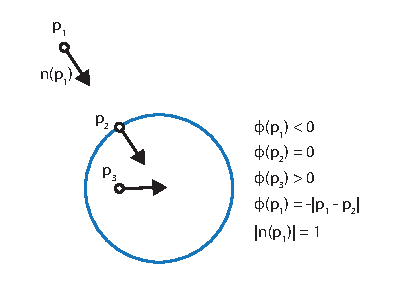
\includegraphics[width=.5 \linewidth]{figures/levelset.pdf}
	\caption{Illustration of the level set in 2D, and its properties.}
	\label{fig:levelset}
\end{figure}

\subsection{Reinitialize signed distance function}
Since the level set only is a sampled signed distance function in practice, a reinitialize operation is used to make sure that the level set is always close to a signed distance function. 
This is done by making sure that the length of the gradient is kept close to 1.
By always having the grid described in this way, it is certain that whenever moving in the direction of the gradient towards the surface with the distance $d$, the closest point on the surface will not change and the distance to the surface is now $d$ less then it was before.

Since the levelset is only a sampled signed distance function in practice, a reinitialize operation is used
\section{Navier-Stokes Equation}
\subsection{Navier-Stokes equation}
The incompressible Navier-Stokes equations in equation (\ref{eq:navierstokes}) offers a way to describe the motion of fluids. 
This equation is the base of most simulations of fluids like water, smoke and fire. 
The equation is made out of a set of partial different equations that describes how the fluid should be behaving trough out the simulation.
\begin{equation}
  \label{eq:navierstokes}
  FIX THIS
\end{equation}
The equations has several parts that represent different physical behaviors of the fluid. 
In the equation, $\vec{u}$ represents the velocity of the fluid.


\subsection{Self-Advection}
In order to completely solve the Navier-Stokes equations, an equation on the following from must first be worked out:
\begin{equation}\label{eq:advect}\frac{\partial q}{\partial t} +\nabla q \cdot \vec{u}= 0\end{equation}
Where \begin{math}q= q(t,\vec{x})\end{math} being some quantity, moving with the velocity field of the fluid, \begin{math}\vec{u}\end{math}, at a certain time \begin{math}t\end{math} and point \begin{math}\vec{x}\end{math} in space. L.h.s in eq. \ref{eq:advect} is also what defines the material derivative, denoted using capital D:
\begin{equation}\frac{Dq}{Dt} = \frac{\partial q}{\partial t} +\nabla q \cdot \vec{u}\end{equation}
The material derivative describes the change of a quantity in a velocity field. An equation using the material derivative is called an advection equation and since the material being advected is the velocity field itself, \begin{math}q = \vec{u}(t,\vec{x})\end{math} eq. \ref{eq:self-advect} is often referred to as Self Advection.
\begin{equation}\label{eq:self-advect}\frac{\partial u}{\partial t} +\nabla u \cdot \vec{u}= 0\end{equation}
From the Eulerian perspective, which is mainly used in this report, we are observing fixed points in space and tracing the change of velocity at these points, while the Lagrangian point of view is focusing on a fixed set of particles and tracing their trajectory (position). Equation \ref{eq:self-advect} states that the velocity is only changing at a location due to movement/replacement of quantity, or more easily explained in Lagrangian terms, the particles are not changing their velocity to any external force, just moving with the flow. The Lagrangian reasoning is fundamental to a commonly used method to find a numerical solution to equation \ref{eq:self-advect} as described in more detail in section \ref{sec:self-advection-implementation}.

\subsection{External forces}
When fire is simulated as it would appear on earth, it is affected by the environment that it is in. 
The characteristics of a lit candle is caused by gravity, combined with boyancy that makes the flame rise and flicker. 
As the air around the flame increases in temperature the hot air rises, causing an upward motion to the flame.
If a fire is lit in space with no gravity acting on it, it would take the shape of a sphere.

\subsection{Projection}
The last step in solving the Navier-Stokes equation is the pressure step, which is also sometimes called the projection step, by its linear algebraic properties of a projection. This step enforces that the velocity field is divergence free, and therefore incompressible, by calculating a pressure field \emph{p} which satisfies this property, eq. X (navierstokes pressure + divergensfritt). 

This can be done by using the Helmholtz-Hodge decomposition theorem which states that a vector field $\vec{v}$ can be expressed as a sum of two vector fields, one curl free $\vec{v_{cf}}$ and one divergence free $\vec{v_{df}}$, eq. x. If $\vec{v}$ is then set as the Ve and Vdf as the requested velocity field Vreq and then set vcf as dt * Delta P / phi, it is possible to reorder Eq helm holtz to a Eq which looks like a euler integration of Ve with the Gradient of P, Eq reorder. 

Eq Helm holtz. v = vcf  + vdf
Eq Helm holz2 Ve = dt * Delta P / phi + Vreq ? 
Eq Vreq = Ve - dt Delta P / phi

It is still two unkowns in Eq Vreq which is one to many to be able to solve this equation. But since Vreq is divergence free it is possible to rule it out by apply the divergence operator V on both sides in Eq helm 2. This results in a possion equation x, which is possible to solve. 

Poission. Eq


\subsection{Boundary Conditions}
When solving the projection step of the Navier-Stokes equation, there are two different types of boundary conditions that need to be enforced in order for the fluid to interact with e.g walls of other solid objects. These conditions can be seen as constraints that rule out unwanted solutions for the partial PDE of the projection step. The first type of boundary condition is the \emph{Dirichlet boundary condition}. It simply states that any partial velocity vector component that points into a grid cell marked as solid is set to have a velocity of zero for that component.

\begin{equation}
\label{eq:dirichlet}
V \cdot n = 0
\end{equation}

In equation (\ref{eq:dirichlet}) \emph{V} is the velocity vector, and \emph{n} is the boundary surface normal. This boundary condition is enforced for the velocity field before and after the projection step. This results in that no velocity vectors will point into grid cells marked as solids.

The second boundary condition is the \emph{Neumann boundary condition} (\ref{eq:neumann}) and it ensures that there is no change of flow between fluid cells and cells marked as solid. The condition is enforced when building the linear equation system during the projection step. The connection between a fluid cell and a neighbouring solid cell is removed by entering a zero-value in the correct location in the diagonal matrix, thus ensuring that no exchange of fluid or change of flow will occur between the cells.

\begin{equation}
\label{eq:neumann}
\frac{\partial V}{\partial n} = 0
\end{equation}
\section{MAC Grid}
\begin{figure}[h!]
\label{fig:mac-grid}
\centering
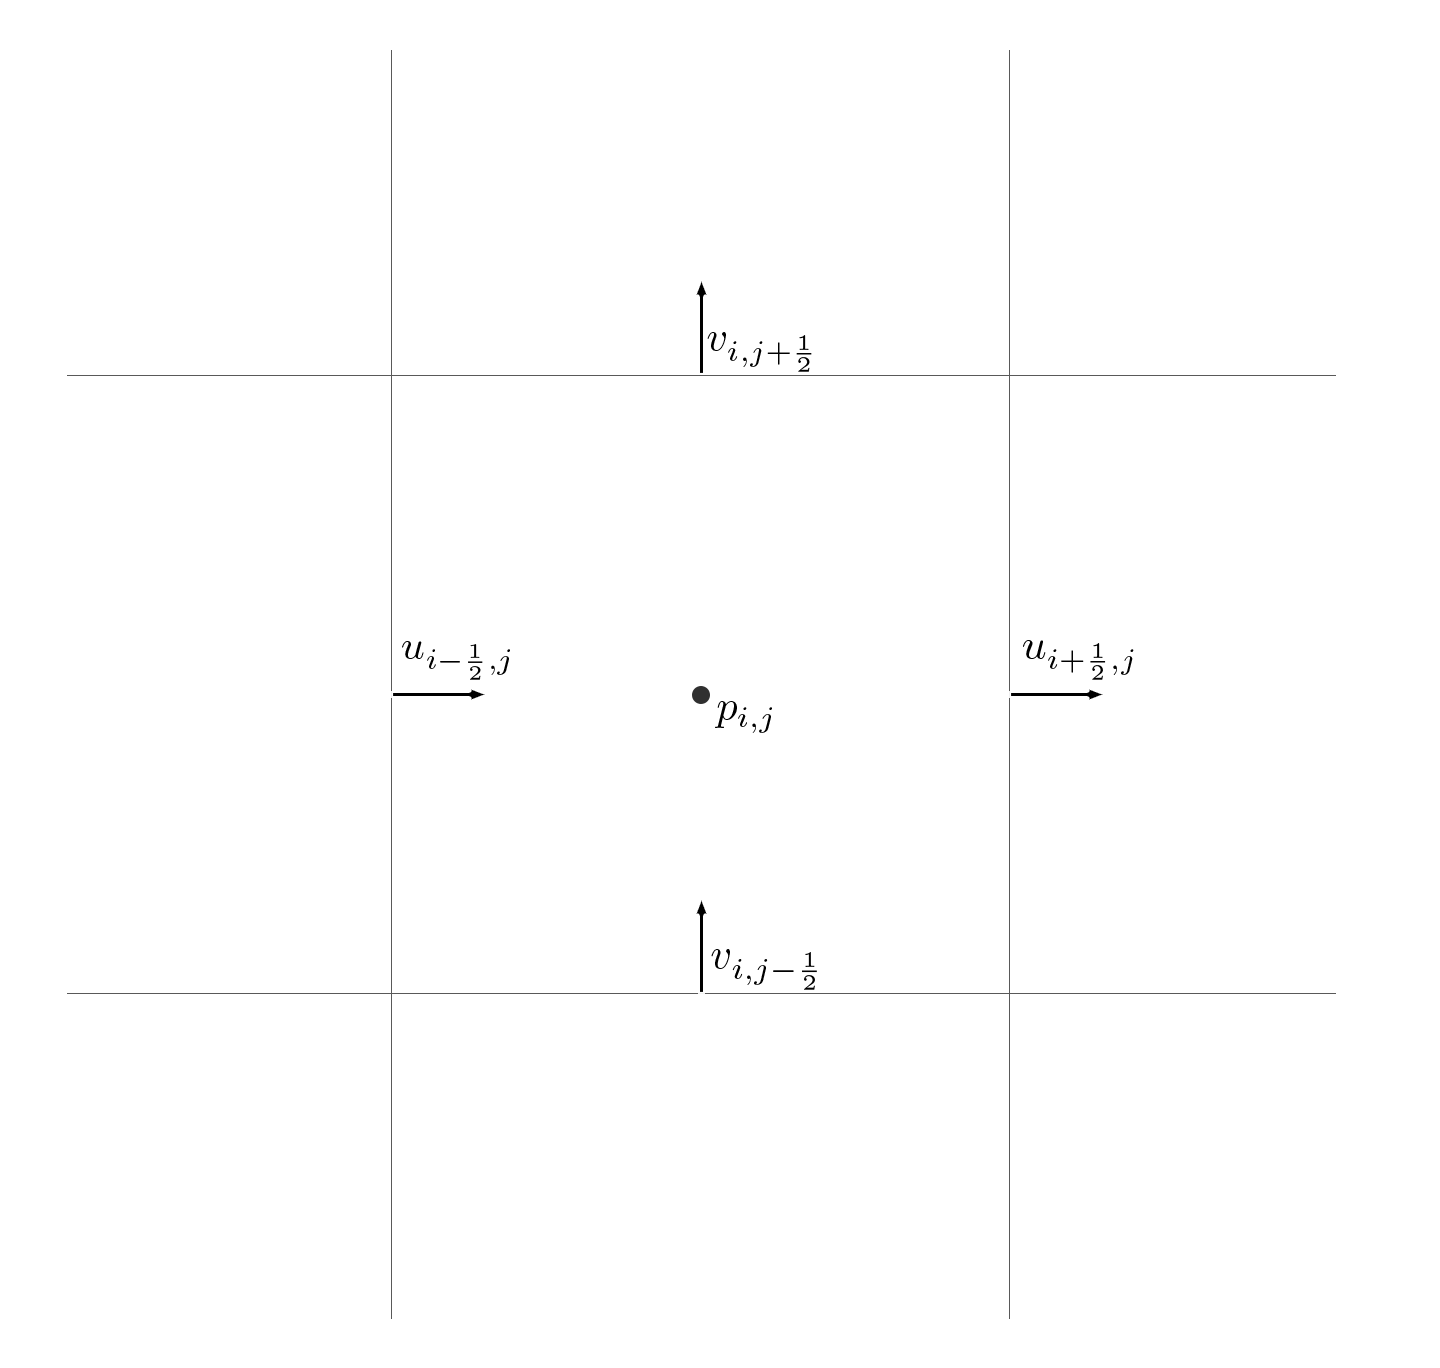
\includegraphics[width=0.6\textwidth]{mac.png}
\caption{2D MAC grid, $p$ is pressure, $u$ and $v$ are velocity components. Half indices are used for illustrative purposes, an implementation should use whole indices.}
\end{figure}

In order to discretize the navier-stokes equations spatially, a technique called MAC (Marker And Cell) is often used. Space is quantified in equally sized cells, sampled quantities such as velocity components and pressure are spread out at different locations in the grid, see fig. \ref{fig:mac-grid}. The pressure is stored in the center of each cell and the velocity is split componentwise and placed at cell faces orthogonal to its direction. 
The placement of velocity vectors and pressure might seem a bit odd but makes the central difference accurate for the pressure gradient and velocity divergence \cite{bridson}, it's easy to find out how much is flowing in or out of a cell which is essential when doing the pressure update. 

A less appealing consequence on the other hand is that a velocity vector can not be accessed directly, it requires interpolation each time since the components are separated. Additional properties might be stored in the grid depending on the type of fluid being simulated, in the case of a fire simulation where buoyancy is a distinguishing feature that can be mimicked by evaluating the local temperature difference, temperature can be stored in the cell center. To track the interface between the blue-core and hot gaseous medium the level-set method is used. The ghost fluid method described in more detail in \ref{sec:method_two_phase_flow} requires a duplicate of each velocity component to account for discontinuous density at the fuel interface.



\section{Rendering}
We are using a ray casting method for rendering our fire. The ray caster collects temperatures over the scene as samples and transform them into a color for each pixel using black-body radiation. The rendering part of the project is a separate work and is included in Appendix A for further reading.

\chapter{Method}
\section{MAC Grid}
The grid is stored as a 1D array of size \begin{math}N\end{math} where \begin{math}N_x*N_y*N_z\end{math} is the number of cells in dimension \begin{math}x\end{math}, \begin{math}y\end{math} and \begin{math}z\end{math}. To access a grid index \begin{math}(i,j,k)\end{math} a transformation from 3D to a 1D array index is made using the following formula:
 \begin{equation} 
 f_{1D}(i,j,k) = i + jN_x + kN_xN_y 
 \end{equation}
To avoid the half indices introduced in fig. \ref{fig:mac-grid}, the following convention is used:  
\begin{align*}
 u_{i-\frac{1}{2},j,k} & =  u[f_{1D}(i,j,k)] 			\\
 u_{i+\frac{1}{2},j,k} & =  u[f_{1D}(i+1,j,k)] 			\\
 v_{i,j-\frac{1}{2},k} & =  v[f_{1D}(i,j,k)] 			\\
 v_{i,j+\frac{1}{2},k} & =  v[f_{1D}(i,j+1,k)] 			\\
 w_{i,j,k-\frac{1}{2}} & =  w[f_{1D}(i,j,k)] 			\\
 w_{i,j,k+\frac{1}{2}} & =  w[f_{1D}(i,j,k+1)] 		
 \end{align*}

Note that $u$,$v$ and $w$ represent different dimensions and could have different lengths $N$, more specifically:
 \begin{align*}
N_u & = (N_x+1)*N_y*N_z			\\
N_v & = N_x*(N_y+1)*N_z			\\
N_w & = N_x*N_y*(N_z+1)				
 \end{align*}
\subsection{Two Phase Flow}
The ghost fluid method requires extra caution when velocities at arbitrary points are evaluated. If the point is close to the interface chances are at least one velocity value is on the other side of the interface when interpolating. The balance equations in section (X.X), are used to enforce mass conservation. In practice, a second velocity field \begin{math}\vec{u}^{ G}\end{math} ("ghost values") is used in parallel to the original velocity field \begin{math}\vec{u}\end{math}. The ghost values are found using the adjusted velocity values described by following equation:
\begin{align}
\Delta V  & = (\frac{\rho_{fuel}}{\rho_{burnt}} - 1)S \\
\end{align}
Where $\rho $ is the density of the fluid, the difference in density between burnt and fuel is what causes the reaction at the flame front. $S$ is the speed in which the fuel is burning, a typical value is about 0.5 m/s. In general $ \hat n$ is the normal pointing from the fluid region to the burnt region, in this case it's the normal of the level-set $ \phi $.
\begin{equation}
    \vec{u}^{G}(\vec{x})= 
\begin{cases}
    \vec{u}(\vec{x})-\Delta V \hat{n},& \text{if } \phi (\vec{x}) \geq 0\\
    \vec{u}(\vec{x})+\Delta V \hat{n},                    & \text{otherwise}
\end{cases}
\end{equation}
In practice this can be done once at the beginning of the simulation by storing the ghost values in second grid or on the fly during simulation to save space. No matter what implementation is used it boils down to a simple check of the level set sign whether the point being used for interpolation is in the same kind of medium (burnt or fuel) and picking the value from same grid if the medium is the same, or choosing the ghost value otherwise. 
\section{Navier-Stokes}
\subsection{Self-Advection}
Where more renowned methods of solving differential equations are failing to find a numerical solution to equation \ref{eq:self-advect} (such as forward Euler for the time derivative and central difference for the spatial derivative\footnote{Which is unconditionally unstable for any \begin{math}\Delta t\end{math} (bridson p.28).}), a method called semi-Lagrangian method is often used to ensure unconditional stability. As the name implies, it is motivated by taking a Lagrangian viewpoint (which treats the fluid as a set of finite particles) in order to aid the Eulerian grid based approach. Consider a particle at  \begin{math}\vec{x}\end{math}, with velocity \begin{math}\vec{u}(\vec{x}) = \frac{d\vec{x}}{dt}\end{math}. If the particle started from grid location \begin{math}\vec{x}_G\end{math} and ended up at \begin{math}\vec{x}_P\end{math} after time step \begin{math}\Delta t \end{math}, assuming constant velocity we have that: 
\begin{equation}
\vec{u}(t,\vec{x}_G) = \vec{u}(t+\Delta t,\vec{x}_P)  
\end{equation}
The same argument can be made backwards: there exists a particle at \begin{math}\vec{x}_{P_1} \end{math} that will end up at grid location \begin{math}\vec{x}_{G_1}\end{math}, finding \begin{math}\vec{x}_{P_1}\end{math} is done simply by tracing the current velocity field backwards in time and evaluating the velocity field at that point. Using simple Euler integration gives: 
%\begin{equation}
	\begin{align}
					      \label{eq:lagrangian}\vec{x_{P_1}}  & =    \vec{x_{G_1}} -  \Delta t \vec{u}(\vec{x_{G_1}})  \\ 
		\vec{u}(t + \Delta t,\vec{x}_{G_1}) &  =    \vec{u}(t,\vec{x}_{P_1}) 
	\end{align}
%\end{equation}
\begin{math} \vec{x_{P_1}} \end{math} is not very likely to be directly at a known grid point, so in order to find \begin{math} \vec{u}(\vec{x_{P_1}}) \end{math} some kind of interpolation has to be used. Both trilinear and cubic interpolation was experimented with, but trilinear interpolation was showed to be adequate for convincing visual results. 
\subsection{External forces}
External forces are handeled in a quite straight forward way. 
For each point in the grid all forces are calculated and added together. 
After that we calculate the new velocity by integrating the force.
The gravitational force is applied uniformly over all grid points that has fluid in them.
Bouyancy is described by a simple model that is directly connected to the temperature in each grid point.
We define it as equation \ref{eq:navierstokes}.
The vector $z$ is a unit vector pointing upward. 
\begin{equation}
\label{eq:buoyancy}
f_{buoy} = \alpha(T-T_{air})z
\end{equation}
$\alpha$ is a possitive constant, $T_{air}$ is the ambient temperature of the room and $T$ is the temperature. 
\subsection{Vorticity Confinement}
Since we are using grids with finite spacing for our simulation, numerical dissipation will cause non-physical damping of some of the fine detail energy in the simulation such as vortices and small scale turbulence. We can add this missing energy back into our simulation by increasing the speed of existing vortices in the fluid. This method is called vorticity confinement and is implemented as in REF TILL RAPPORT HÄR. First we calculate the curl $\omega$ of the original vector field.
\begin{equation}
\label{eq:vorticity}
\omega = \nabla \times \vec{V}
\end{equation}
We define normalized vorticity vectors $\vec{N}$ that will point from areas with low vorticity towards areas with high vorticity.
\begin{equation}
\label{eq:vort_loc_vec}
\vec{N} = \frac{\nabla |\omega|}{|\nabla |\omega ||}
\end{equation}

The resulting vorticity confinement force $\vec{f}_{vort}$ to be added to the velocity fields can then be calculated using these vorticity location vectors.

\begin{equation}
\label{eq:vort_force}
	\vec{f}_{vort} = \epsilon\Delta x(\vec{N}\times\omega))
\end{equation}

In equation (\ref{eq:vort_force}) $\epsilon$ is some arbitrary scalar to control the magnitude of the vorticity force being added. The dependency on $\Delta x$ ensures that as the grid resolution is refined and $\Delta x$ grows smaller the vorticity confinement force added decreases as well, resulting in the physically correct result being obtained. The resulting force $\vec{f}_{vort}$ is added to the velocity fields as an external force.
\subsection{Projection}
The projection step is a linear operation to update $\vec{u}$ according to the pressure, $p$.
This is done to maintain incompressibility as seen in the Navier-stokes equations, equation \eqref{eq:incompress}, we have to for each timestep compensate for the pressure to make $\vec{u}$ divergence-free.
\begin{equation}
\label{eq:incompress}
	\nabla\cdot \vec{u}= 0
\end{equation}
To retrieve the pressure $p$ we have to solve the equation \eqref{eq:Apb} \cite{bridson}.
\begin{equation}
\label{eq:Apb}
	Ap = b
\end{equation}
Where $A$ is the coefficient matrix, each row corresponds to one cell in the fluid. So for large grids $A$ will be extremly storage dependent. $b$ is a vector with all the negative divergences for each cell of the fluid. 

After $A$ and $b$ are calculated and set they are inserted into a PCG-solver (Preconditioned Conjugate Gradient), to retrieve the pressure vector $p$.
As mentioned earlier, when the new pressure-gradient is retrieved we can for incompressibility calculate the new $\vec{u}$ which will be needed for the next time step.


\section{Advecting level set}
The blue core does not only move with the velocity field $\vec{u_f}$, it is also burning with the speed $S$ in the normal direction. This means that the level set which defines the blue core is advected by the velocity field $\vec{w} = \vec{u_f} + S \vec{n}$, where $\vec{n}$ is calculated using a central difference, eq. \ref{eq:central_diff}.

\begin{equation}
\label{eq:central_diff}
\frac{\partial \phi}{\partial x} \approx \phi_x^\pm = \frac{\phi_{i+1,j,k} - \phi_{i-1,j,k}}{\Delta x }
\end{equation}  

To ensure stability in equation \ref{eq:levelset_advection} \cite{CFL}, the finite difference is calculated using a upwind scheme, eq. \ref{eq:upwind}. eq. \ref{eq:levelset_advection} must also satisfy the time step constraint in eq. \ref{eq:time_constraint}.

\begin{equation}
\label{eq:upwind}
\frac{\partial \phi}{\partial x} \approx \left\{\begin{matrix}
 \phi_x^+ = \frac{\phi_{i+1,j,k} - \phi_{i,j,k}}{\Delta x } & ,\vec{w_x} < 0
\\ 
 \phi_x^- = \frac{\phi_{i+1,j,k} - \phi_{i-1,j,k}}{\Delta x } & ,\vec{w_x} > 0 
\end{matrix}\right.
\end{equation}  

\begin{equation}
\label{eq:time_constraint}
\Delta t < min \left \{ \frac{\Delta x}{ \vec{w_x} }, \frac{\Delta y}{ \vec{w_y} }, \frac{\Delta z}{ \vec{w_z} } \right \}
\end{equation} 

$\vec{n}$ is not assured to be a unit vector since it is a numerical approximation of a signed distance function, $\vec{n}$ is therefore normalized before usage. $\vec{n}$ could even be evaluated as a null vector, in these cases a constant unit vector $(0, 1, 0)$ which is pointing upwards, is used.

\subsection{Extrapolation}

When accessing values outside the grid, extrapolation is needed to find out the value of the signed distance function, e.g. when calculating the finite difference. Some easy ways to do this is by using a constant value or by finding the closest real value to it. More sophisticated methods is to make the value fulfil the properties of a signed distance function as described in \cite{bridson}. The method below is a more simple way to mimic a signed distance function. 

Find the closest real position $p_r$ to the position $p_e$. The extrapolated value $\phi_e$ is then calculated using $\phi(\vec{p_r})$ subtracted with the distance between $p_r$ and $p_e$, eq. \ref{eq:levelset_extrapolation}. This means that the value is further away from the interface. 

\begin{equation}
\label{eq:levelset_extrapolation}
\phi_e(\vec{p_e}) =  \phi(\vec{p_r}) - \left | p_r - p_e  \right |
\end{equation} 

This solution would be true if the extrapolated value were in the negative normal direction from the real value.

\chapter{Results}
\section{Results}

\begin{table}[H]\footnotesize
\caption{Settings and performance for the figures}
\begin{tabular}{lllllll}
\hline
Figure & $\vec{u}_{fuel}/\vec{u}_{burnt}$ grid & $T$ grid & $T_{ign}/T_{max}$ & $S$ & $\epsilon_{burnt}$ & Simulation/Rendering time (s) \\
\hline
\ref{fig:fire1}      &	30x60x30	&	90x180x90	&	2200/3000	&	0.1	&		60	&	5/64	\\
\ref{fig:fire2}      &	15x30x15	&	90x180x90	&	2200/3000	&	0.1	&		60	&	3/64	\\
\ref{fig:fire3}      &	60x120x60	&	90x180x90	&	2200/3000	&	0.1	&		60	&	30/64	\\
\ref{fig:fire7}      &	30x60x30	&	90x180x90	&	1500/1500	&	0.1	&		60	&	5/64	\\
\ref{fig:fire8}      &	30x60x30	&	90x180x90	&	2200/3000	&	0.25	&	60	&	5/64	\\
\ref{fig:fire9}      &	30x60x30	&	90x180x90	&	2200/3000	&	0.025	&	60	&	5/64	\\
\ref{fig:fire10}     &	30x60x30	&	90x180x90	&	2200/3000	&	0.1		&	100	&	5/64	\\
\hline
\end{tabular}
\end{table}

Common settings for all figures are $\alpha = 0.15$, $\epsilon_{fuel} = 16$,  $\rho_{fuel} = 1.0$, $\rho_{burnt} = 0.01$ and $T_{loss} = 3000$. All figures have been rendered on a computer using a Intel 3770K CPU. 

The fire in the figures shown does not consider the walls as boundaries in this simulation and therefore moves through them. The fuel is injected as a sphere in each frame for all but one of the figures.

\begin{figure}[H]
\centering�
\subfigure[frame 9]{\centering
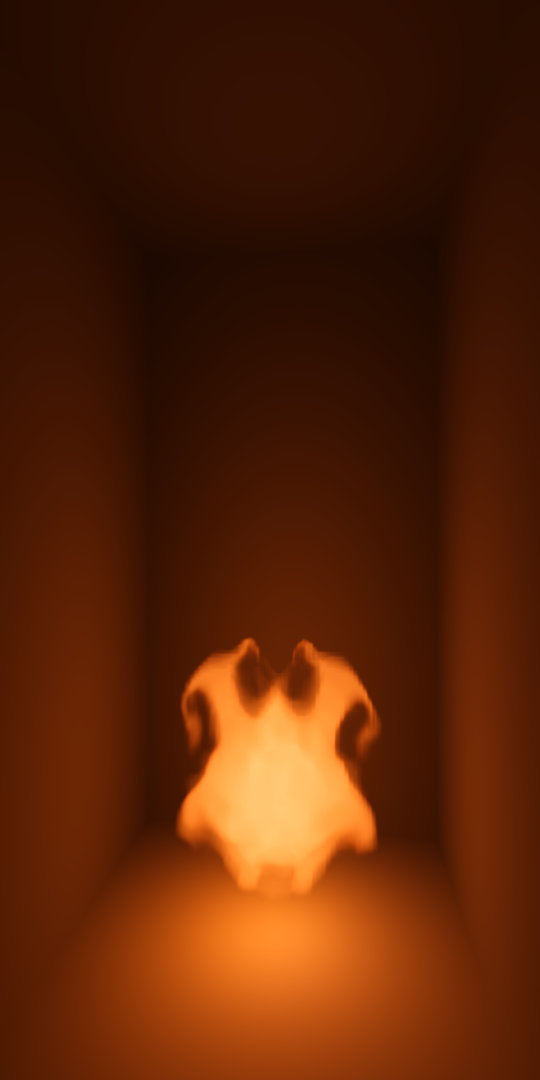
\includegraphics[width=.3 \linewidth]{figures/fire1/9.png}
}
\subfigure[frame 50]{\centering
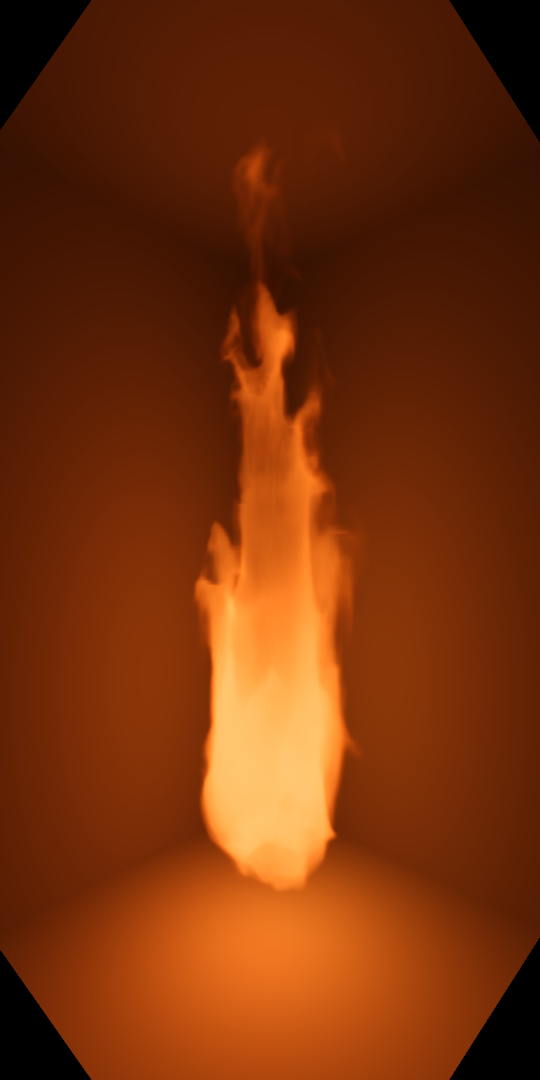
\includegraphics[width=.3\linewidth]{figures/fire1/50.png}
}
\subfigure[frame 144]{\centering
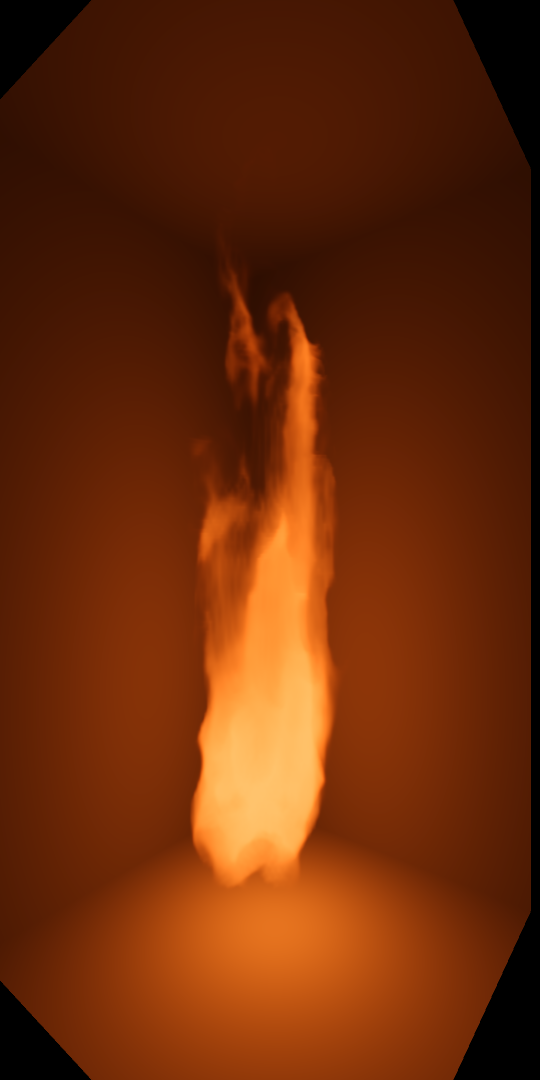
\includegraphics[width=.3\linewidth]{figures/fire1/144.png}
}
\caption
{
\label{fig:fire1}
The figure shows the result of the settings which are used as reference settings for the rest of the figures.
}
\end{figure}

\begin{figure}[H]
\centering
\subfigure[frame 9]{\centering
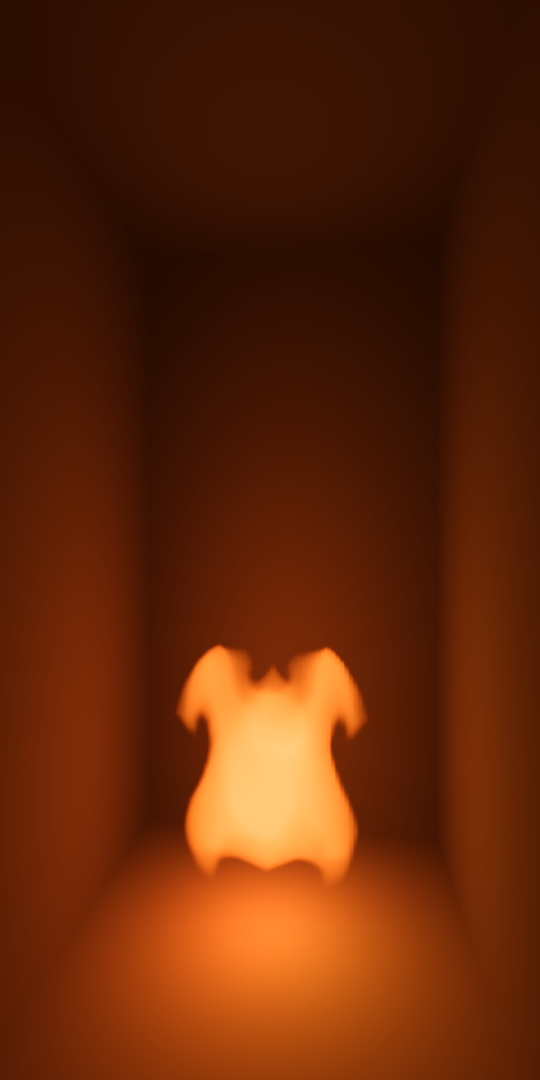
\includegraphics[width=.3 \linewidth]{figures/fire2/9.png}
}
\subfigure[frame 50]{\centering
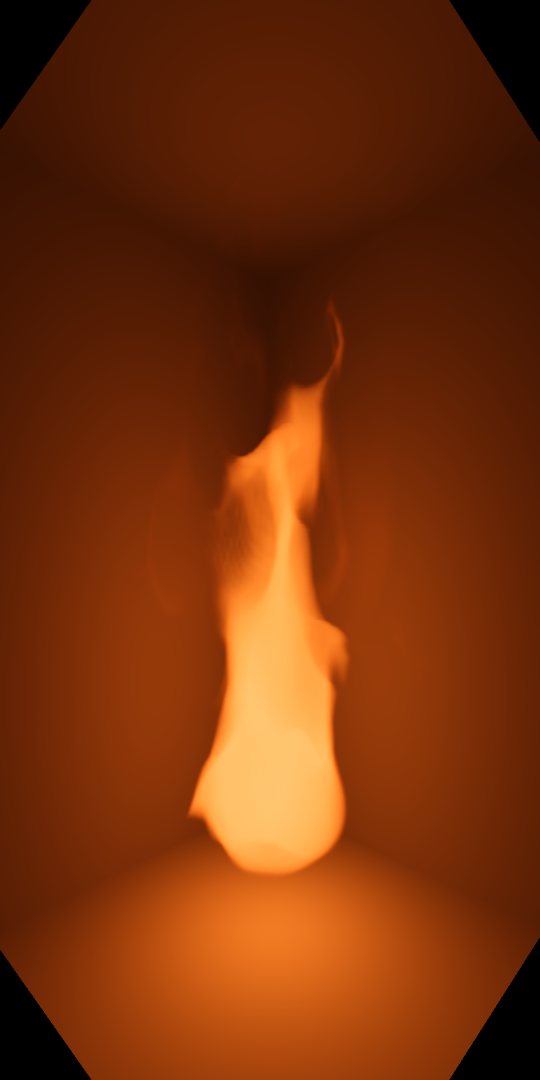
\includegraphics[width=.3\linewidth]{figures/fire2/50.png}
}
\subfigure[frame 144]{\centering
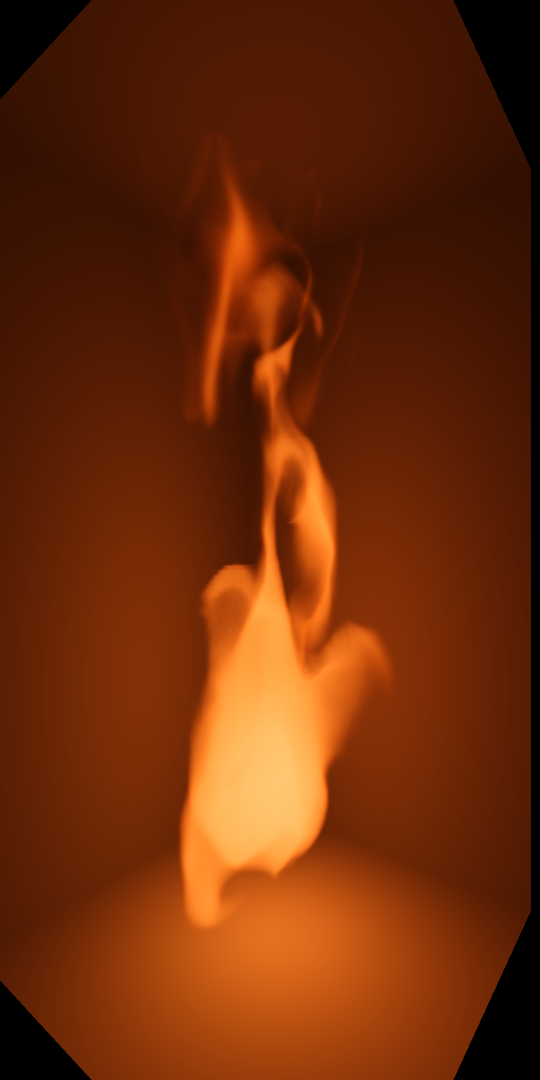
\includegraphics[width=.3\linewidth]{figures/fire2/144.png}
}
\caption
{
\label{fig:fire2}
The velocity grid has half the reference resolution, i.e the simulation has half the resolution.
}
\end{figure} 

\begin{figure}[H]
\centering
\subfigure[frame 9]{\centering
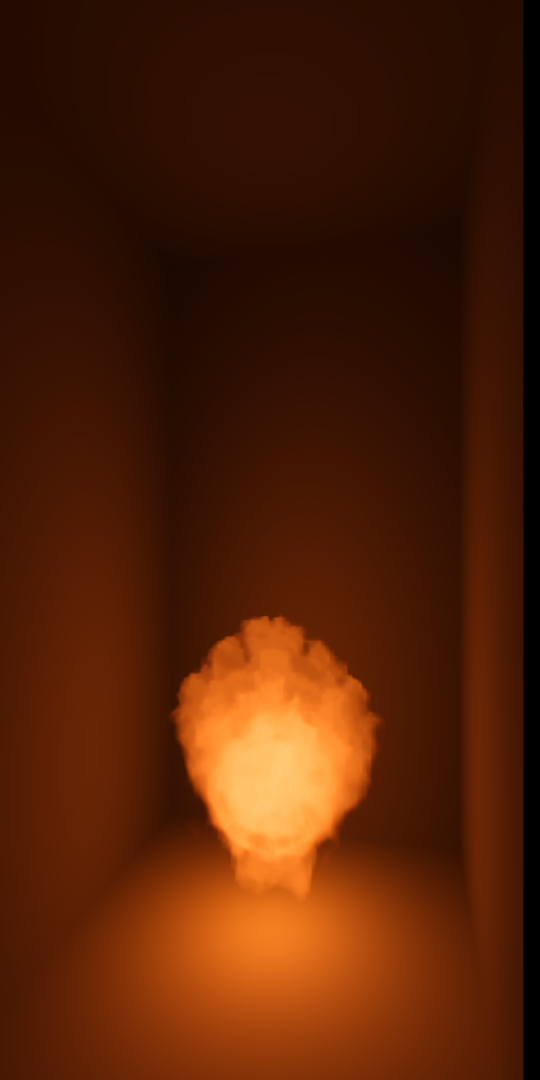
\includegraphics[width=.3 \linewidth]{figures/fire3/9.png}
}
\subfigure[frame 50]{\centering
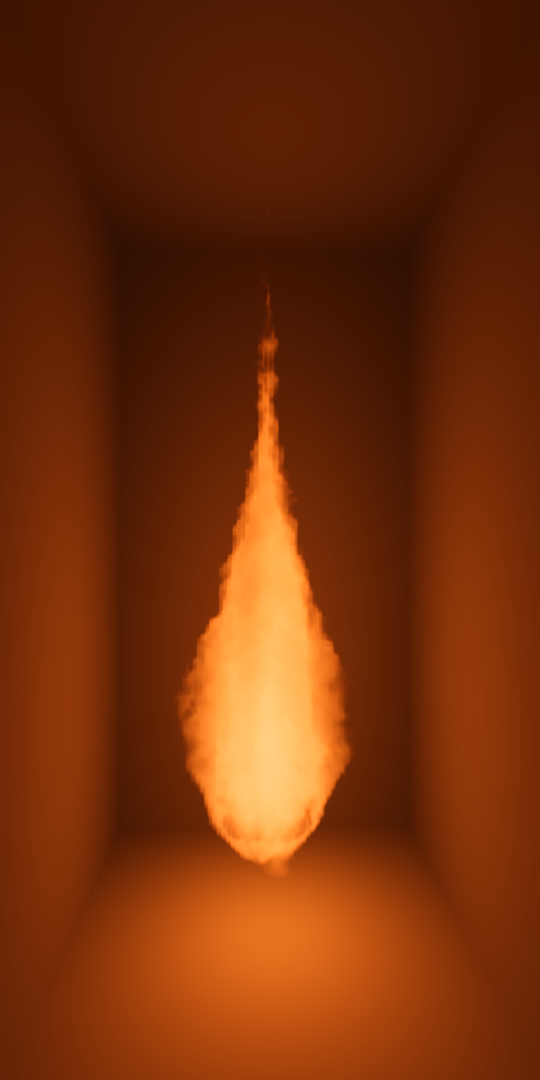
\includegraphics[width=.3\linewidth]{figures/fire3/50.png}
}
\subfigure[frame 144]{\centering
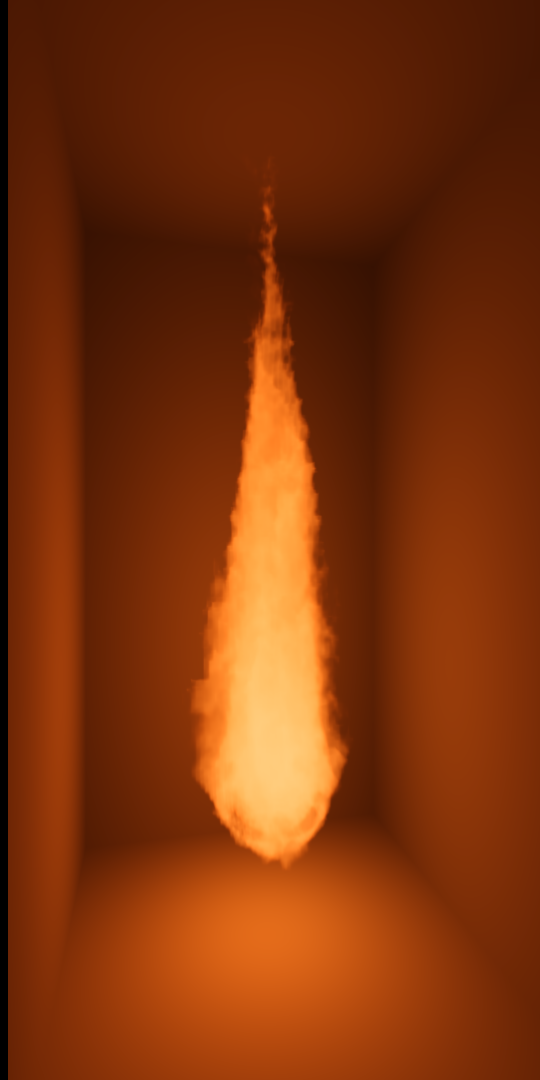
\includegraphics[width=.3\linewidth]{figures/fire3/144.png}
}
\caption
{
\label{fig:fire3}
The velocity grid has twice the reference resolution.
}
\end{figure} 

\begin{figure}[H]
\centering
\subfigure[frame 9]{\centering
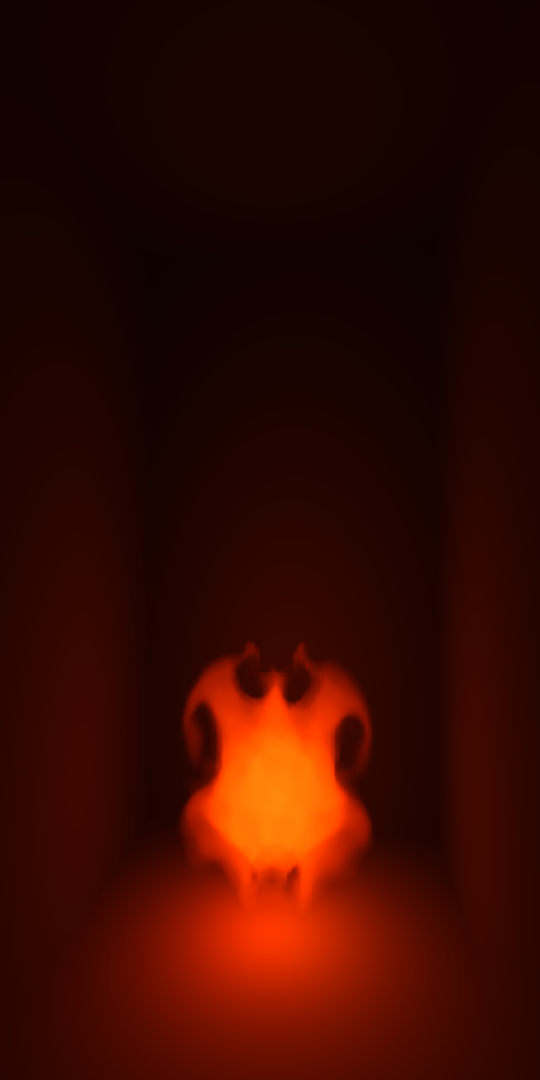
\includegraphics[width=.3 \linewidth]{figures/fire7/9.png}
}
\subfigure[frame 50]{\centering
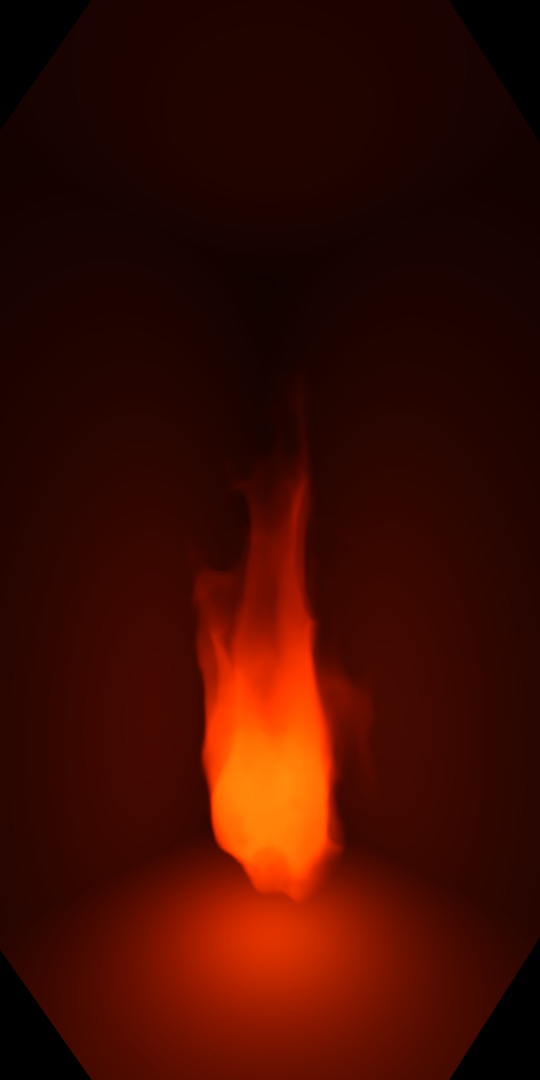
\includegraphics[width=.3\linewidth]{figures/fire7/50.png}
}
\subfigure[frame 144]{\centering
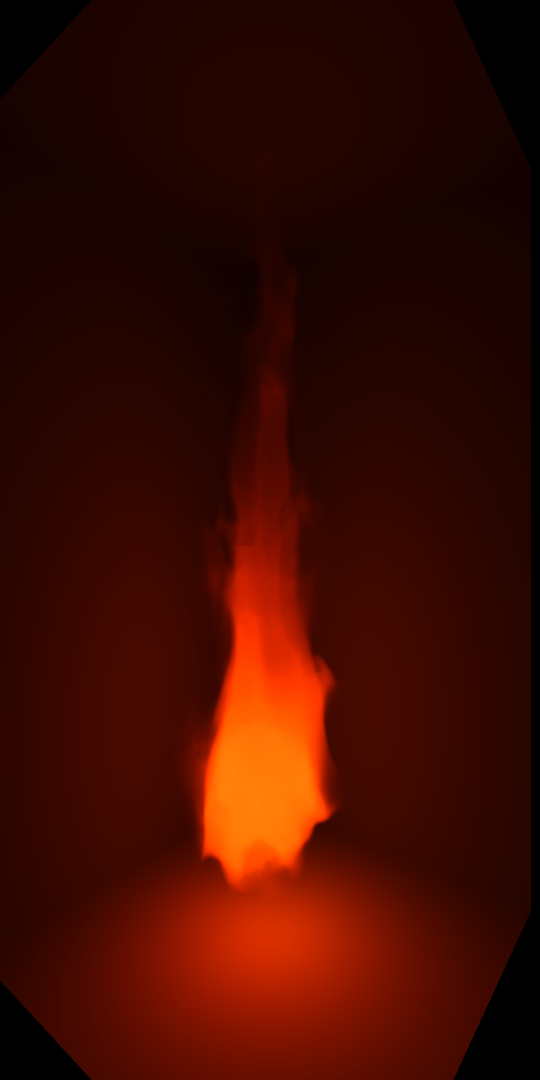
\includegraphics[width=.3\linewidth]{figures/fire7/144.png}
}
\caption
{
\label{fig:fire7}
Using a lower ignition- and max temperature than the reference. The chromatic adaptation constant is set to 1 instead of 100.
}
\end{figure} 

\begin{figure}[H]
\centering
\subfigure[frame 9]{\centering
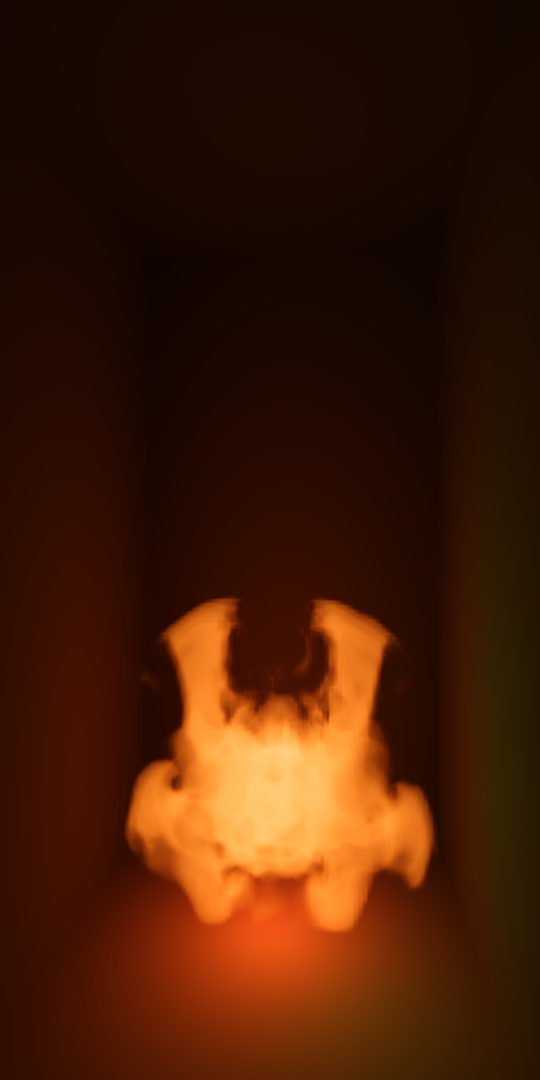
\includegraphics[width=.3 \linewidth]{figures/fire8/9.png}
}
\subfigure[frame 50]{\centering
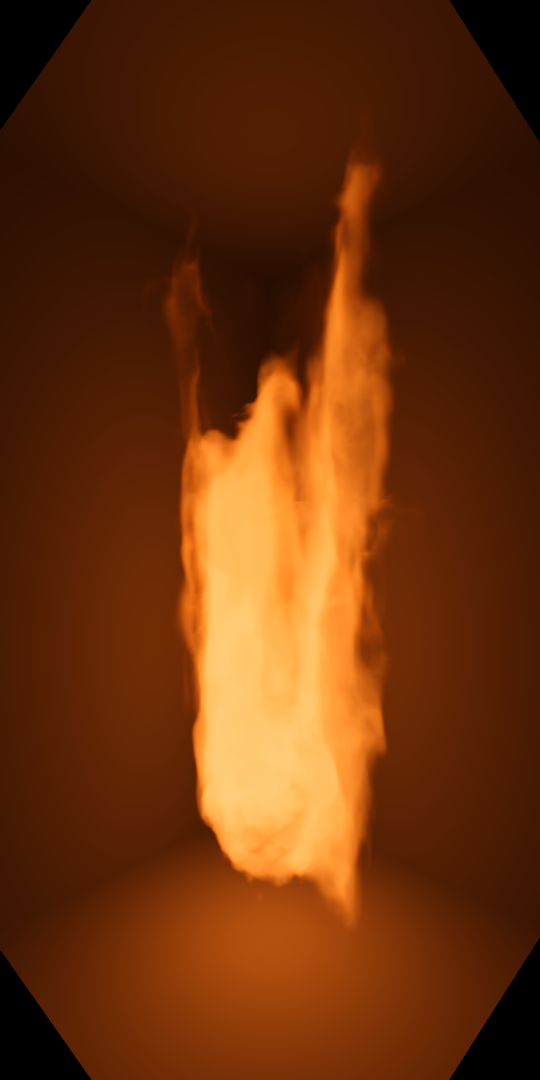
\includegraphics[width=.3\linewidth]{figures/fire8/50.png}
}
\subfigure[frame 144]{\centering
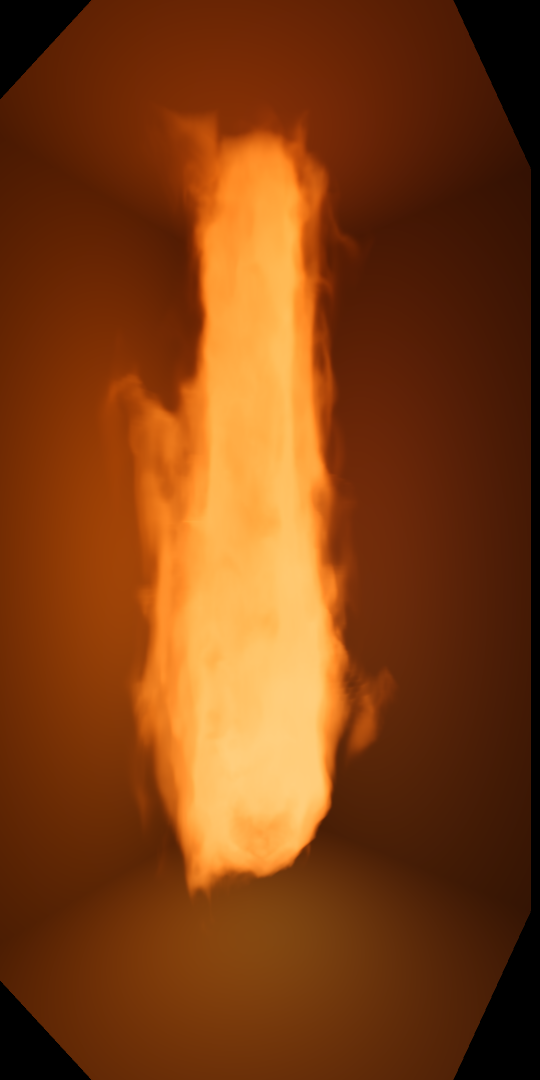
\includegraphics[width=.3\linewidth]{figures/fire8/144.png}
}
\caption
{
\label{fig:fire8}
Using a higher flame speed $S$ than the reference.
}
\end{figure}  

\begin{figure}[H]
\centering
\subfigure[frame 9]{\centering
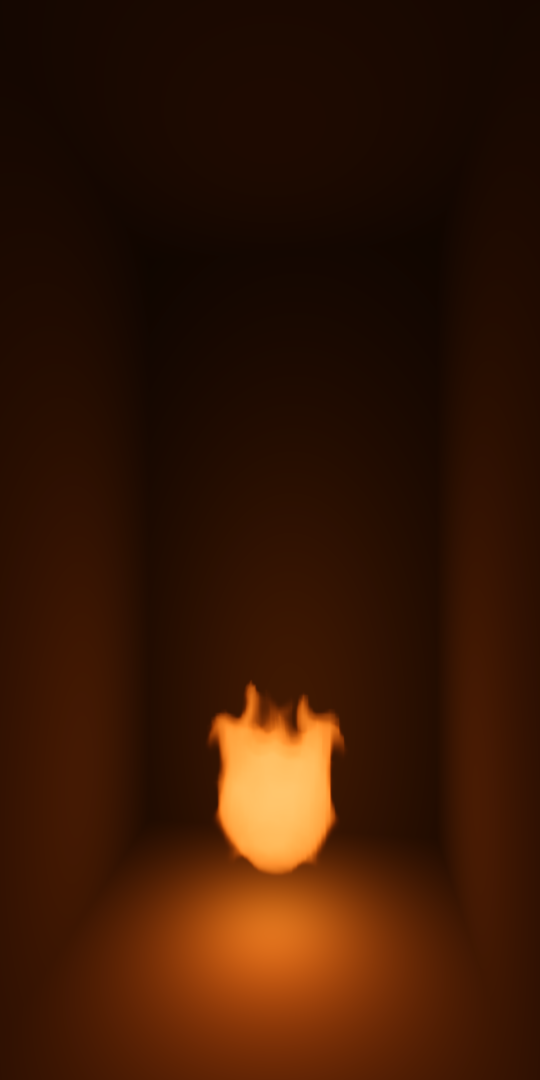
\includegraphics[width=.3 \linewidth]{figures/fire9/9.png}
}
\subfigure[frame 50]{\centering
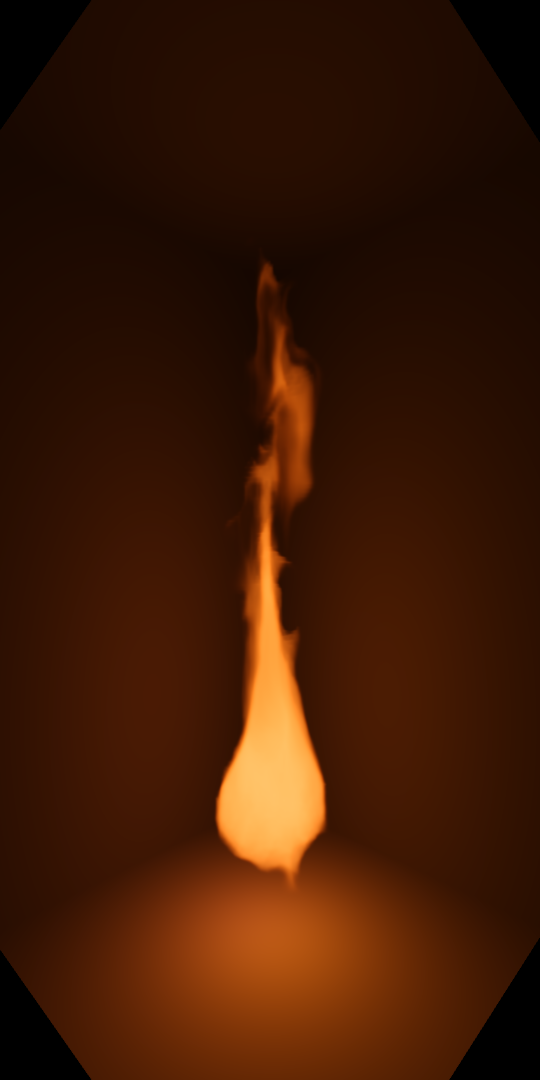
\includegraphics[width=.3\linewidth]{figures/fire9/50.png}
}
\subfigure[frame 144]{\centering
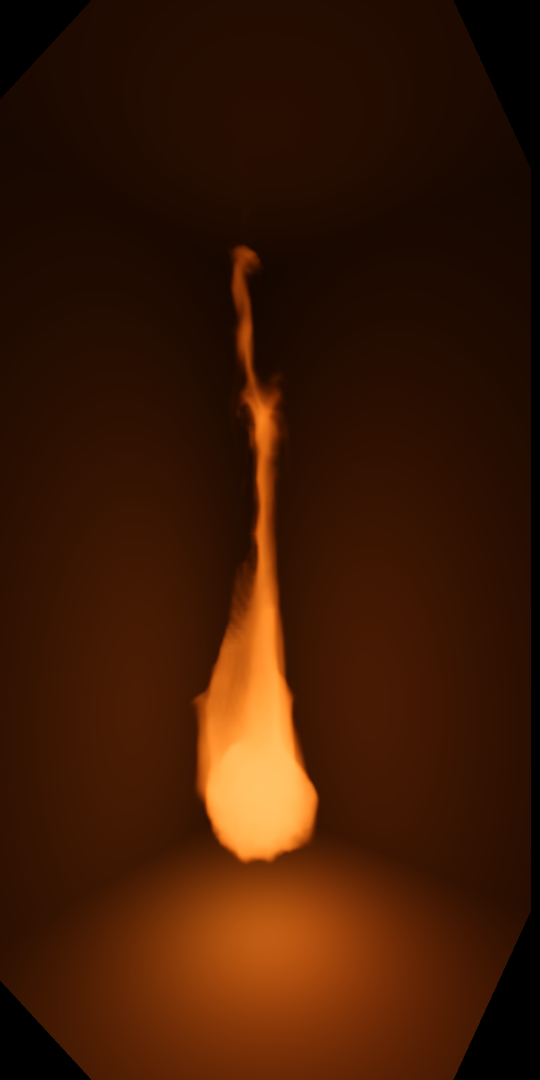
\includegraphics[width=.3\linewidth]{figures/fire9/144.png}
}
\caption
{
\label{fig:fire9}
Using a lower flame speed $S$ than the reference.
}
\end{figure} 

\begin{figure}[H]
\centering
\subfigure[frame 9]{\centering
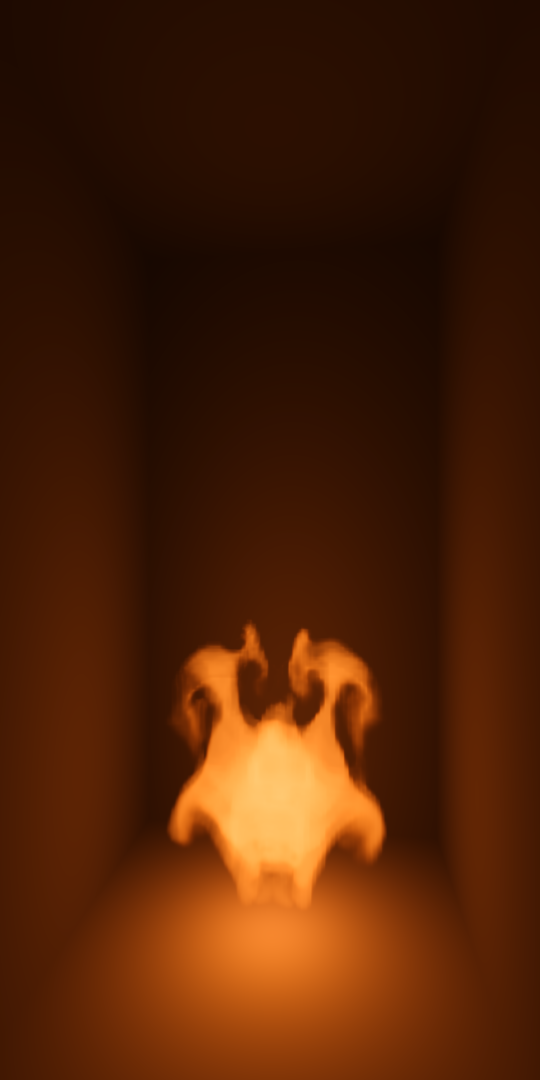
\includegraphics[width=.3 \linewidth]{figures/fire10/9.png}
}
\subfigure[frame 50]{\centering
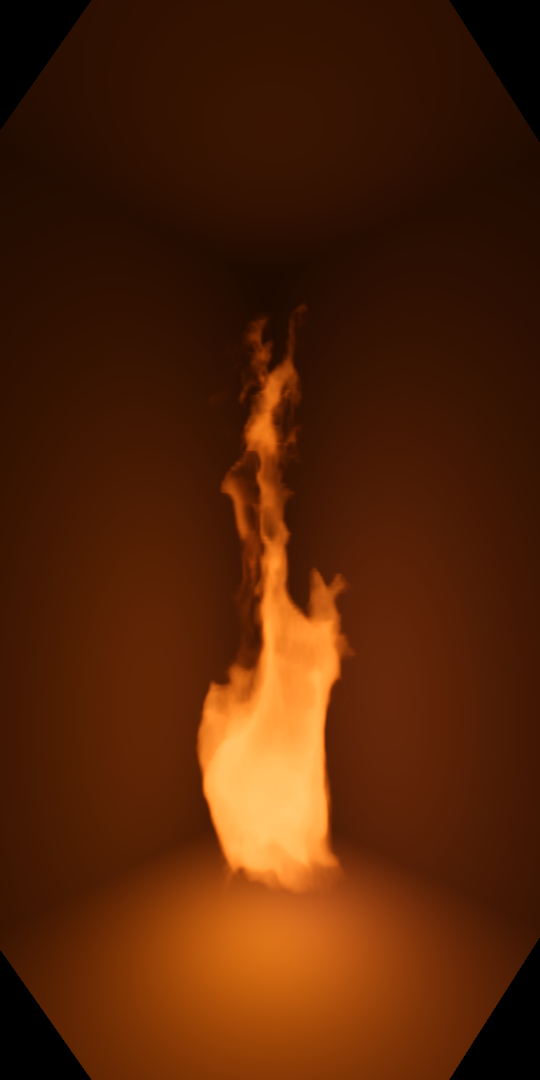
\includegraphics[width=.3\linewidth]{figures/fire10/50.png}
}
\subfigure[frame 144]{\centering
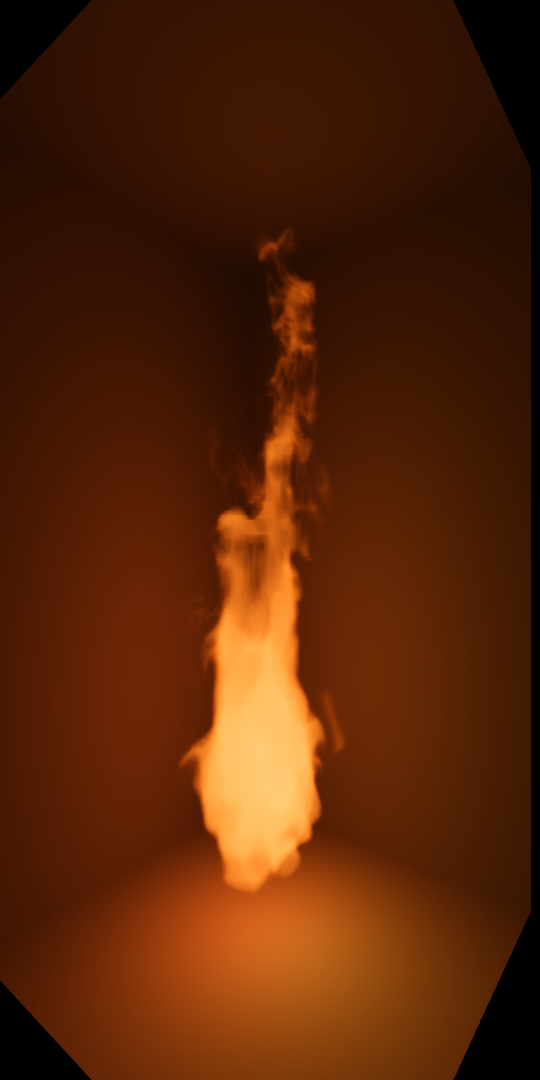
\includegraphics[width=.3\linewidth]{figures/fire10/144.png}
}
\caption
{
\label{fig:fire10}
Using a higher $\epsilon_h$ than the reference.
}
\end{figure} 

\begin{figure}[H]
\centering
\subfigure[frame 5]{\centering
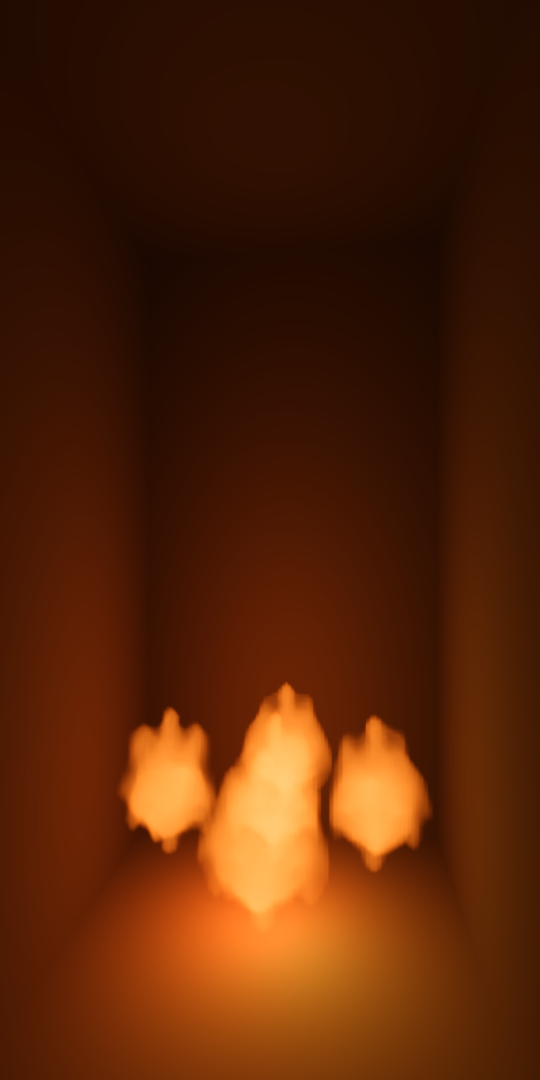
\includegraphics[width=.3 \linewidth]{figures/fire6/5.png}}
\subfigure[frame 99]{\centering
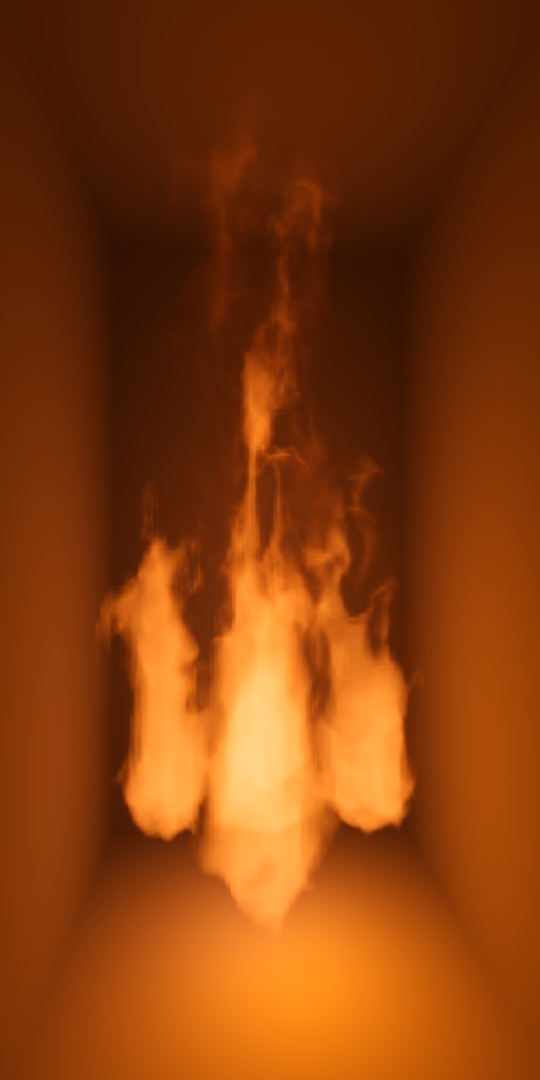
\includegraphics[width=.3\linewidth]{figures/fire6/99.png}}
\caption
{
\label{fig:fire4}
Injecting 5 smaller spheres with fuel instead of one big.
}
\end{figure}  

\begin{figure}[H]
\centering
\subfigure[frame 9]{\centering
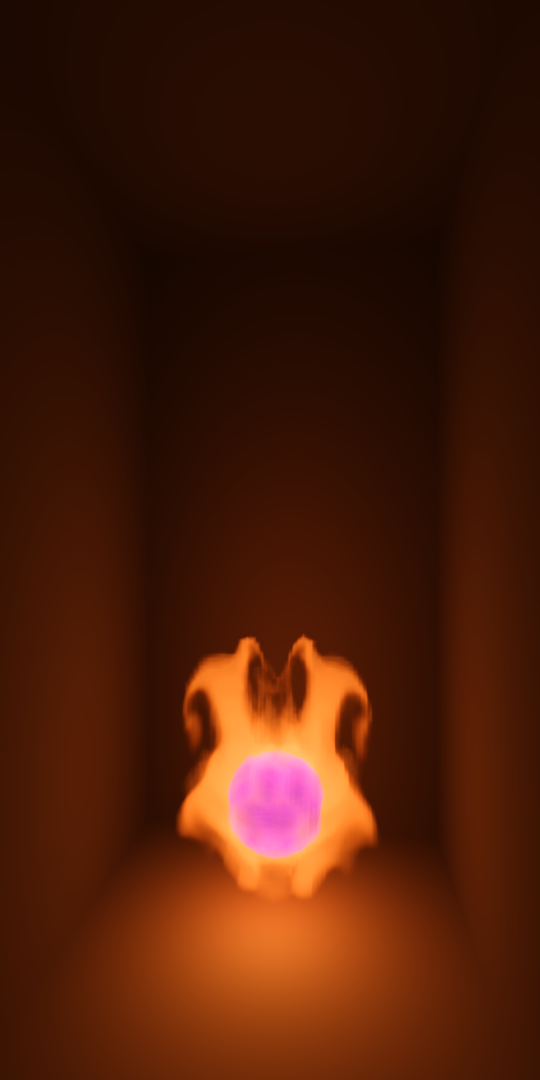
\includegraphics[width=.3 \linewidth]{figures/fire4/9.png}
}
\subfigure[frame 41]{\centering
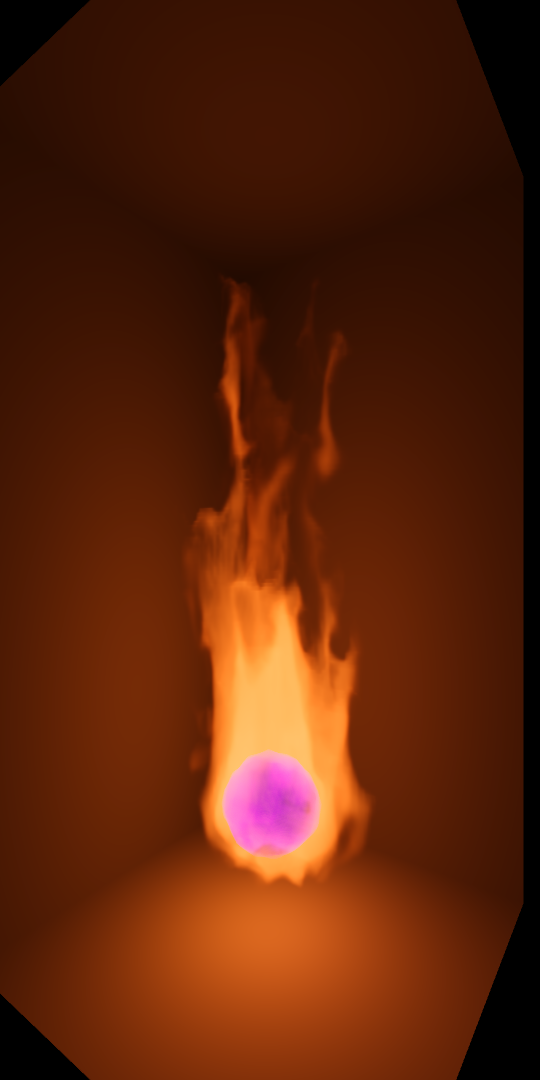
\includegraphics[width=.3\linewidth]{figures/fire4/41.png}
}
\subfigure[frame 50]{\centering
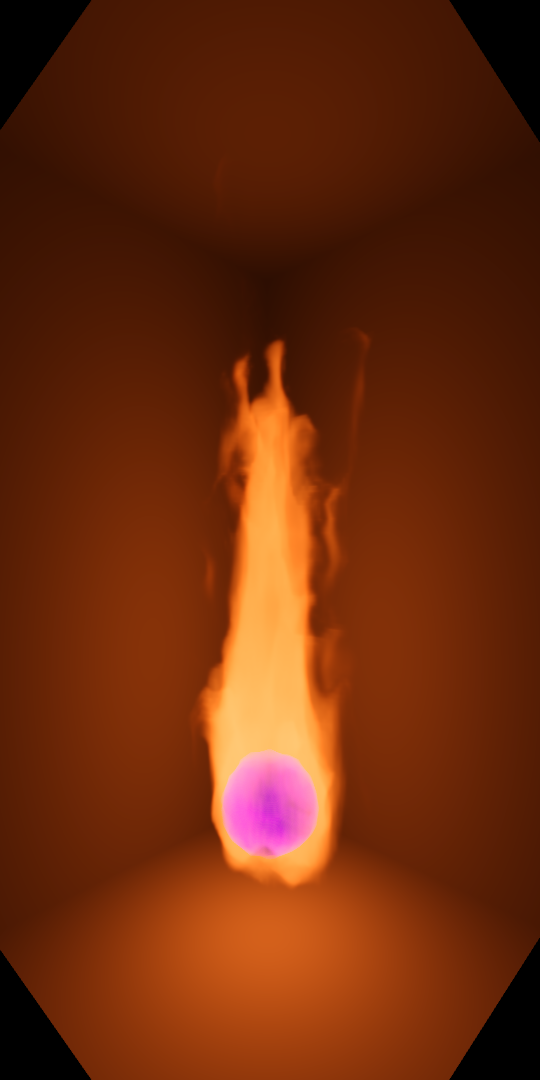
\includegraphics[width=.3\linewidth]{figures/fire4/50.png}
}
\caption
{
\label{fig:fire4}
The blue core converts the radiance from the black body radiation to purple radiance only.   
}
\end{figure}

\begin{figure}[H]
\centering
\subfigure[frame 2]{\centering
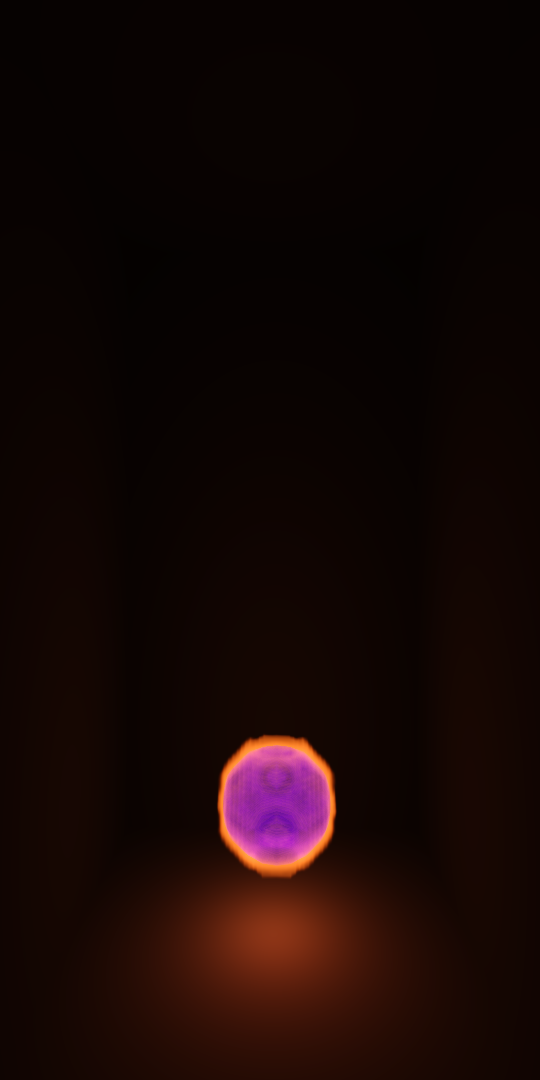
\includegraphics[width=.23 \linewidth]{figures/fire5/2.png}}
\subfigure[frame 9]{\centering
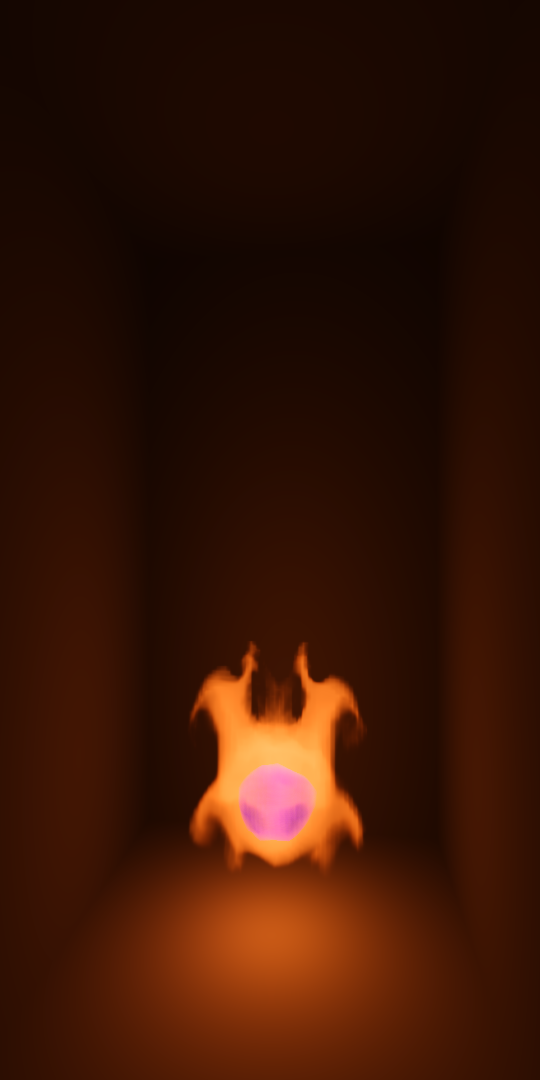
\includegraphics[width=.23\linewidth]{figures/fire5/9.png}}
\subfigure[frame 13]{\centering
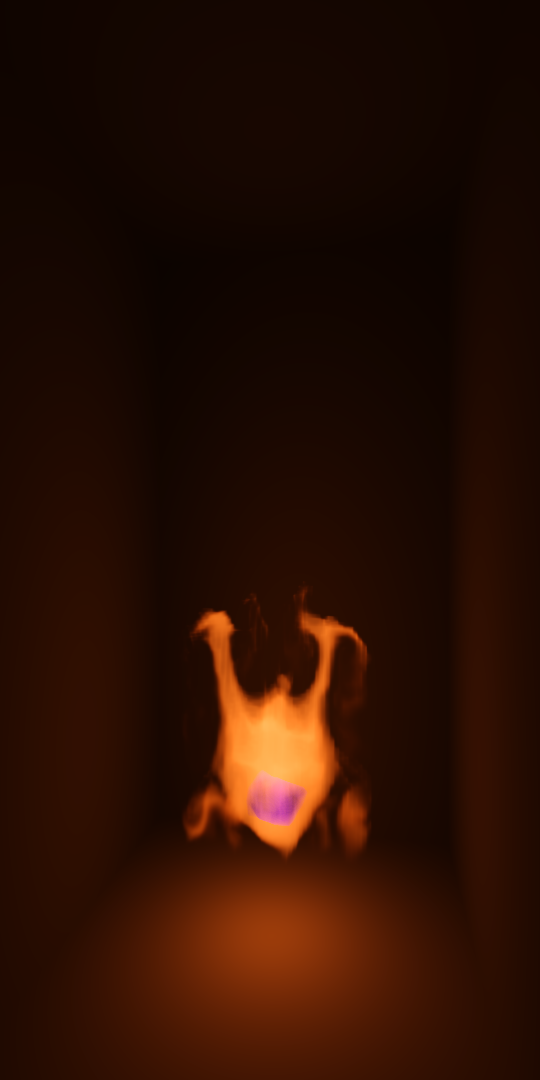
\includegraphics[width=.23\linewidth]{figures/fire5/13.png}}
\subfigure[frame 25]{\centering
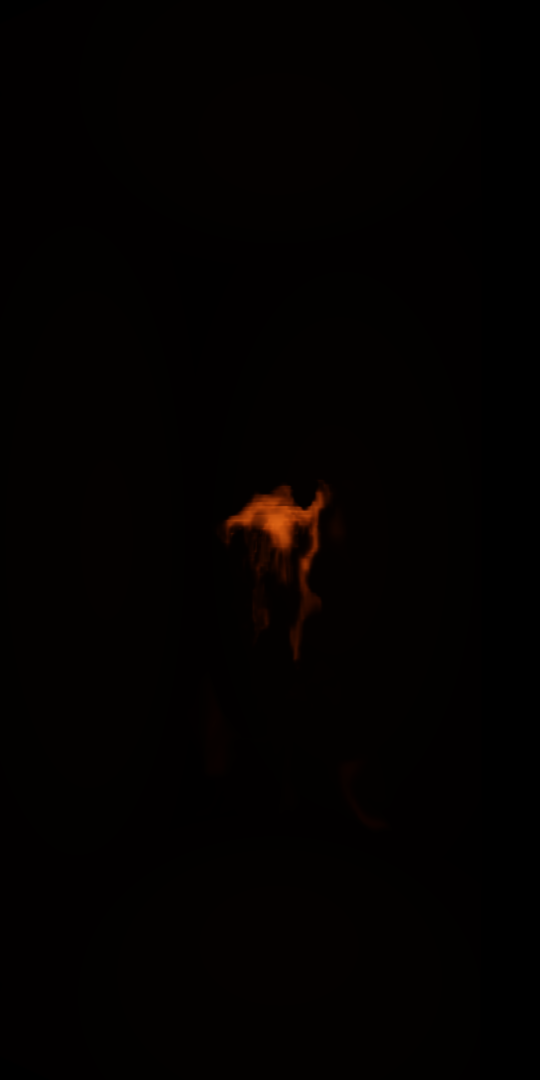
\includegraphics[width=.23\linewidth]{figures/fire5/25.png}}
\caption
{
\label{fig:fire5}
Same as figure \ref{fig:fire5}, but without fuel injection.
}
\end{figure}   

\begin{figure}[H]
\centering
\subfigure[frame 60]{\centering
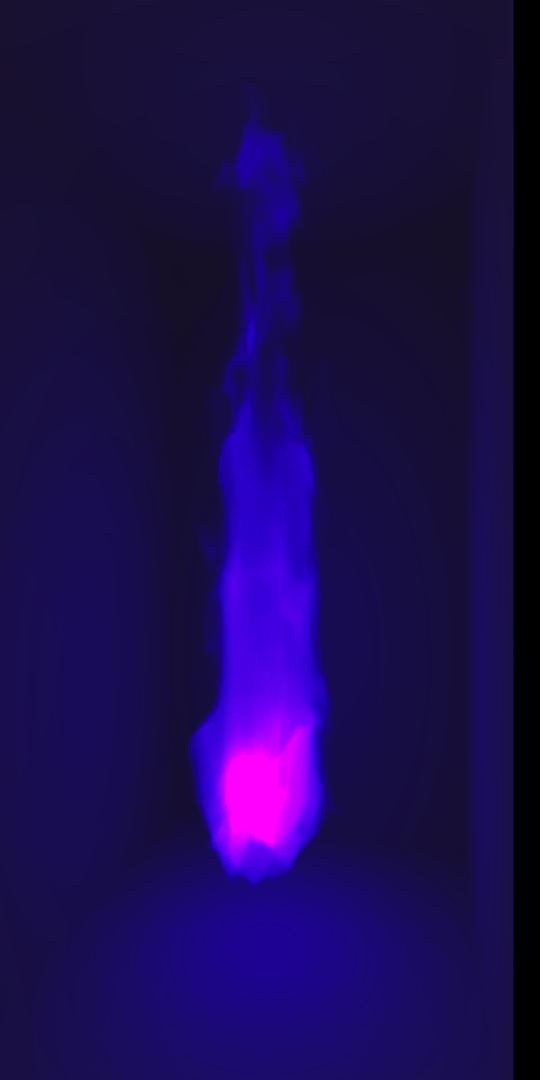
\includegraphics[width=.19 \linewidth]{figures/fire11/60.png}}
\subfigure[frame 68]{\centering
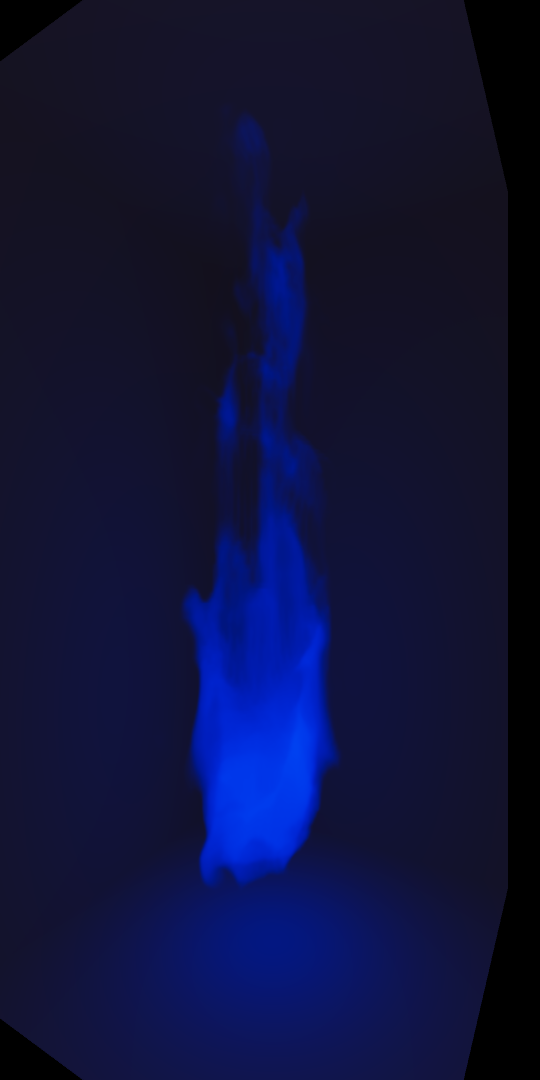
\includegraphics[width=.19\linewidth]{figures/fire11/68.png}}
\subfigure[frame 73]{\centering
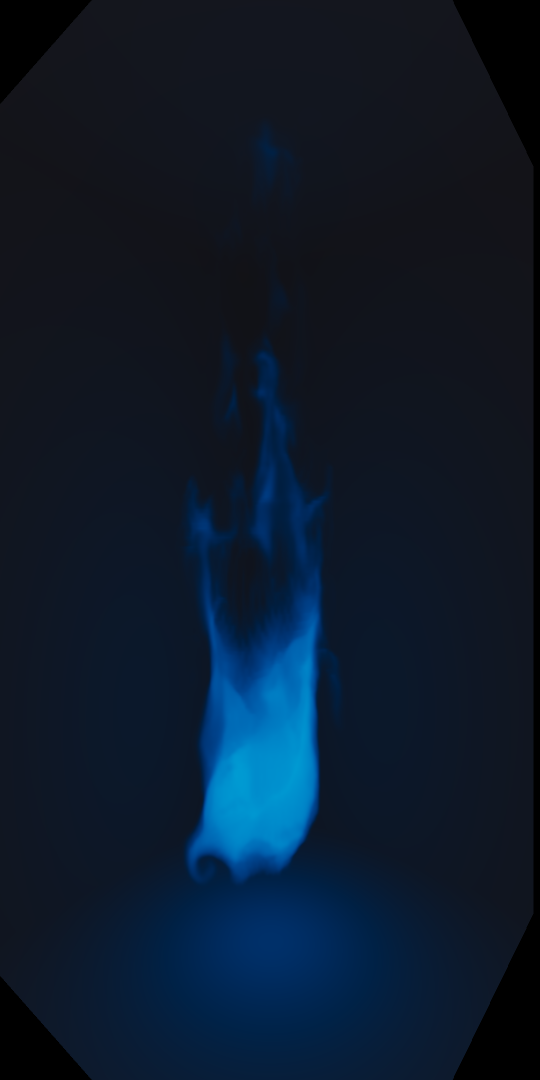
\includegraphics[width=.19\linewidth]{figures/fire11/73.png}}
\subfigure[frame 89]{\centering
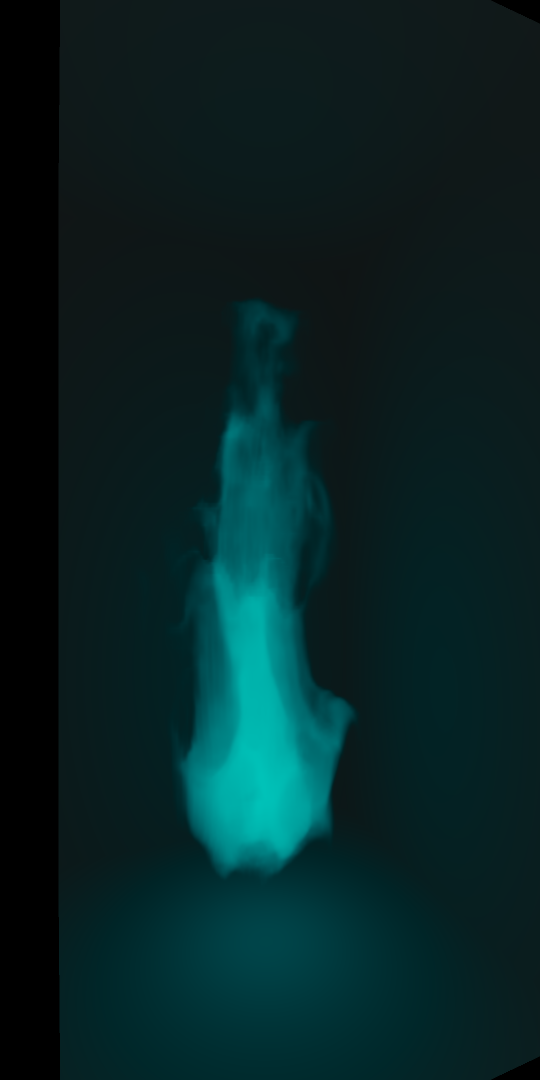
\includegraphics[width=.19\linewidth]{figures/fire11/89.png}}
\subfigure[frame 96]{\centering
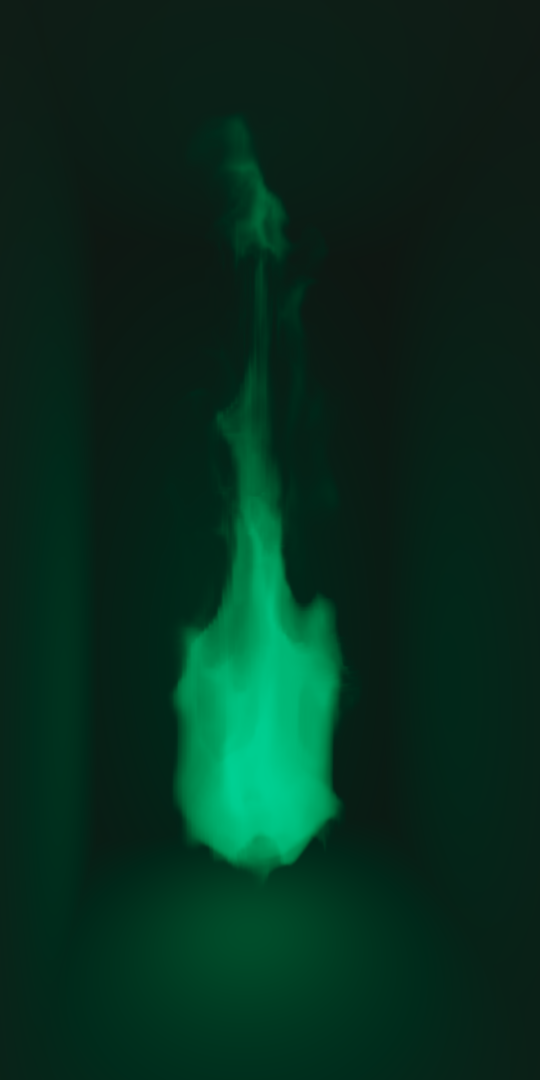
\includegraphics[width=.19\linewidth]{figures/fire11/96.png}}
\subfigure[frame 117]{\centering
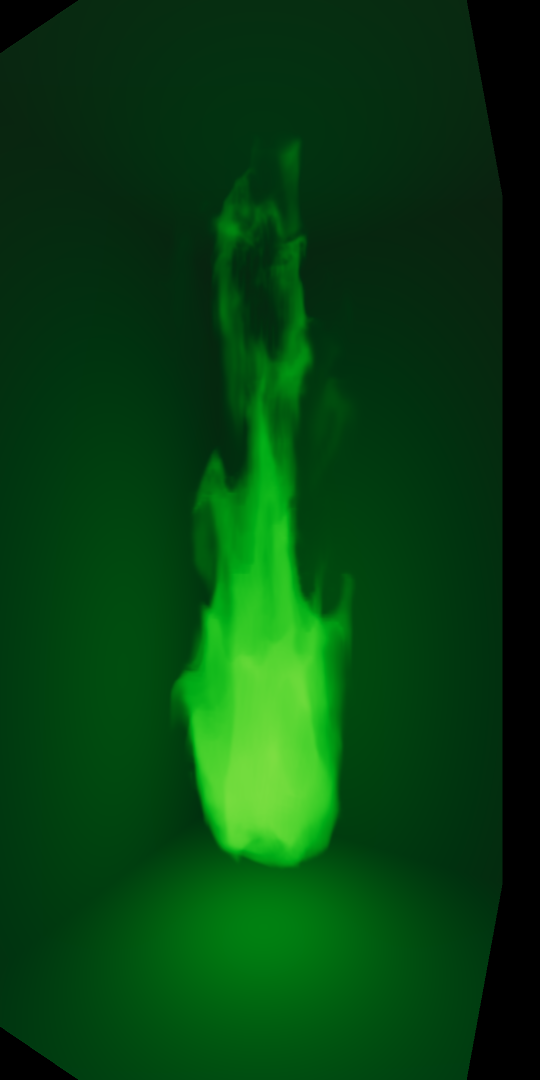
\includegraphics[width=.19\linewidth]{figures/fire11/117.png}}
\subfigure[frame 162]{\centering
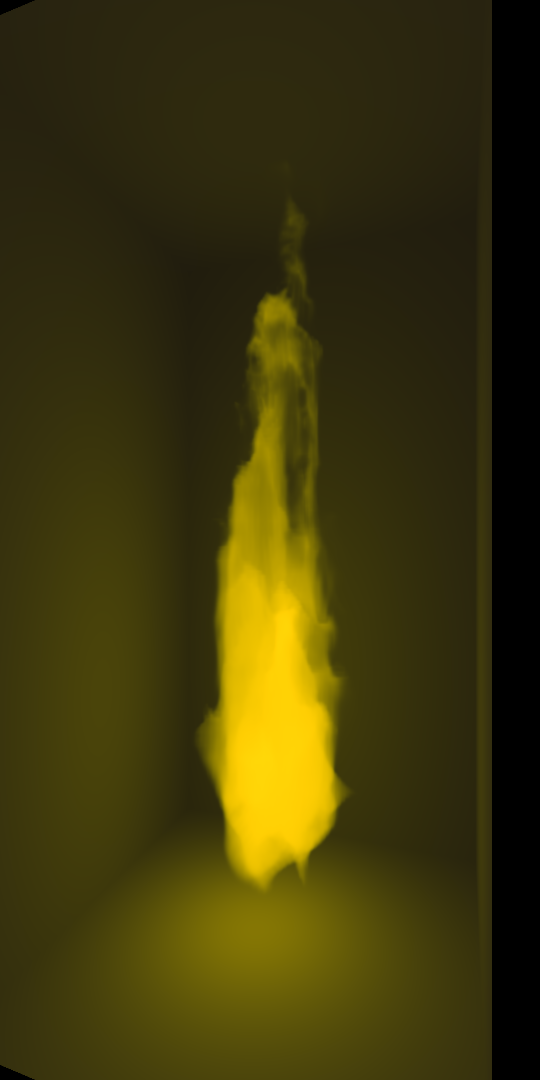
\includegraphics[width=.19\linewidth]{figures/fire11/162.png}}
\subfigure[frame 178]{\centering
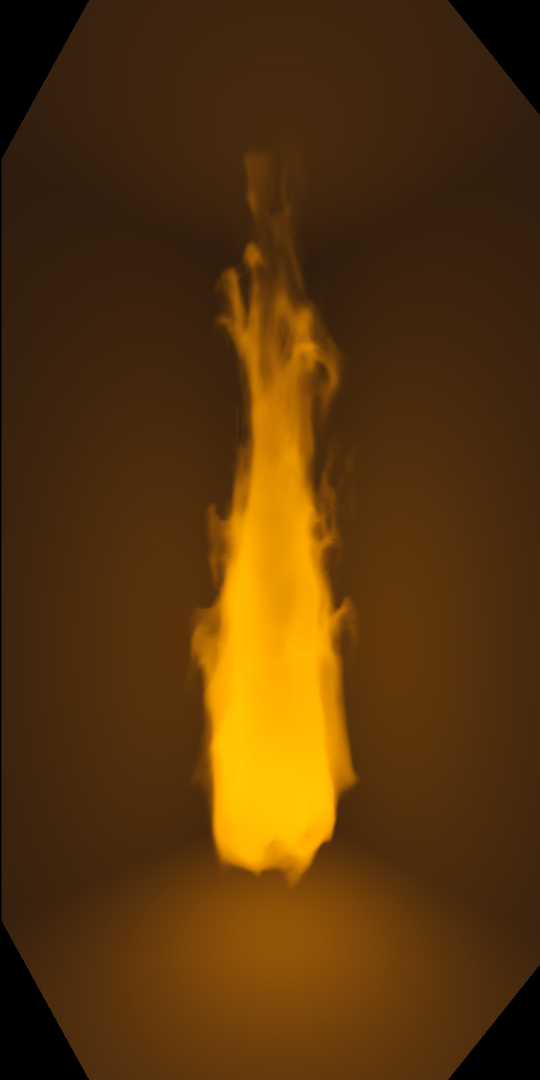
\includegraphics[width=.19\linewidth]{figures/fire11/178.png}}
\subfigure[frame 189]{\centering
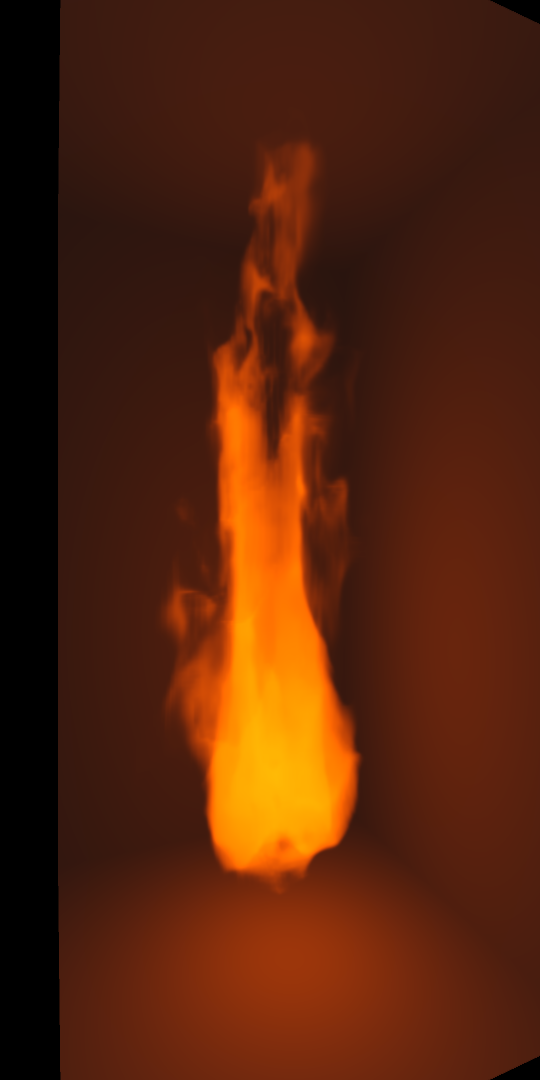
\includegraphics[width=.19\linewidth]{figures/fire11/189.png}}
\subfigure[frame 209]{\centering
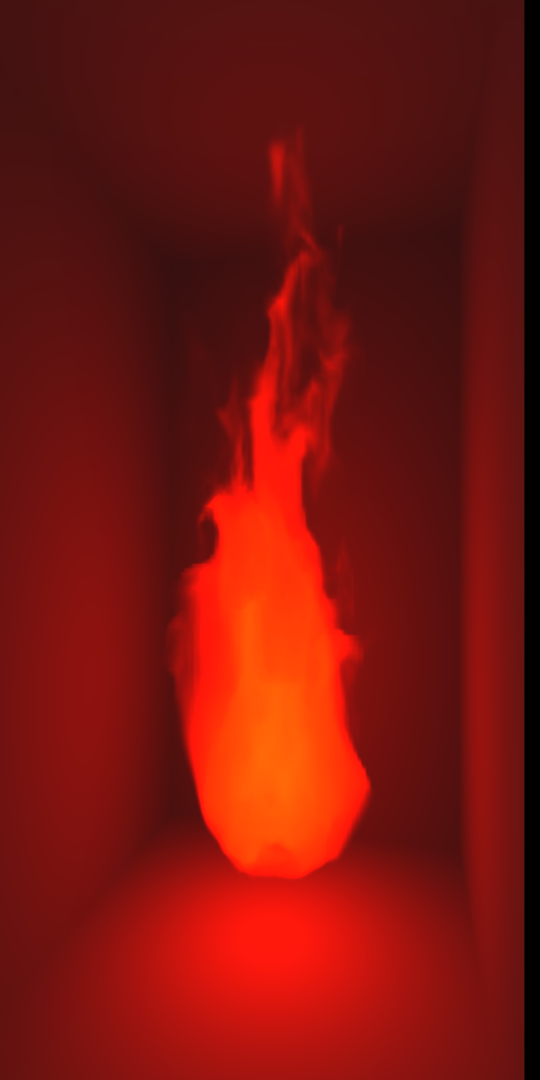
\includegraphics[width=.19\linewidth]{figures/fire11/209.png}}
\caption
{
\label{fig:fire5}
The black body only emits radiance for one wavelength at the time.
}
\end{figure} 

\begin{figure}[H]
\centering
\subfigure[frame 4]{\centering
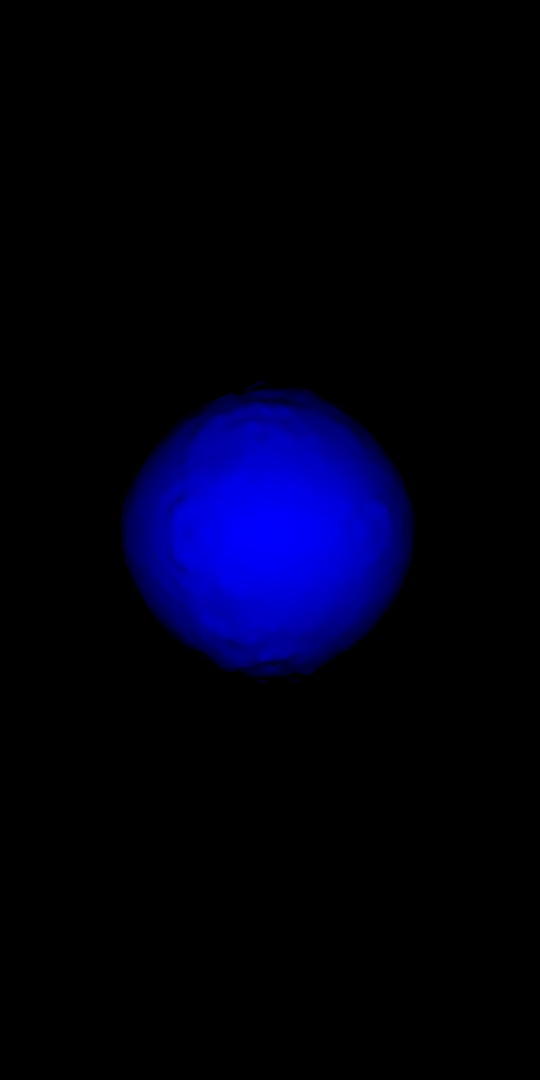
\includegraphics[width=.3 \linewidth]{figures/bluecore/4.png}}
\subfigure[frame 8]{\centering
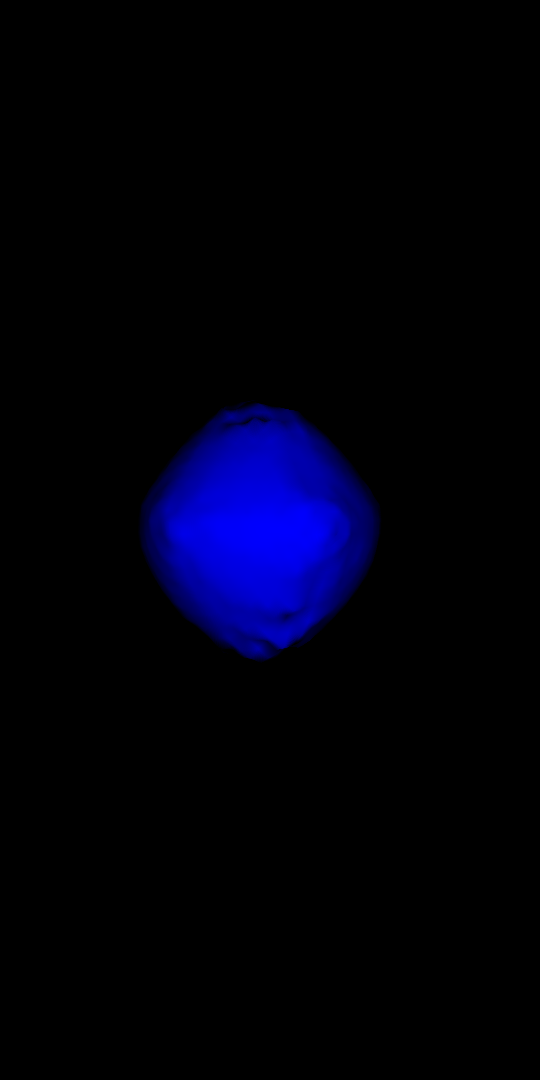
\includegraphics[width=.3\linewidth]{figures/bluecore/8.png}}
\subfigure[frame 20]{\centering
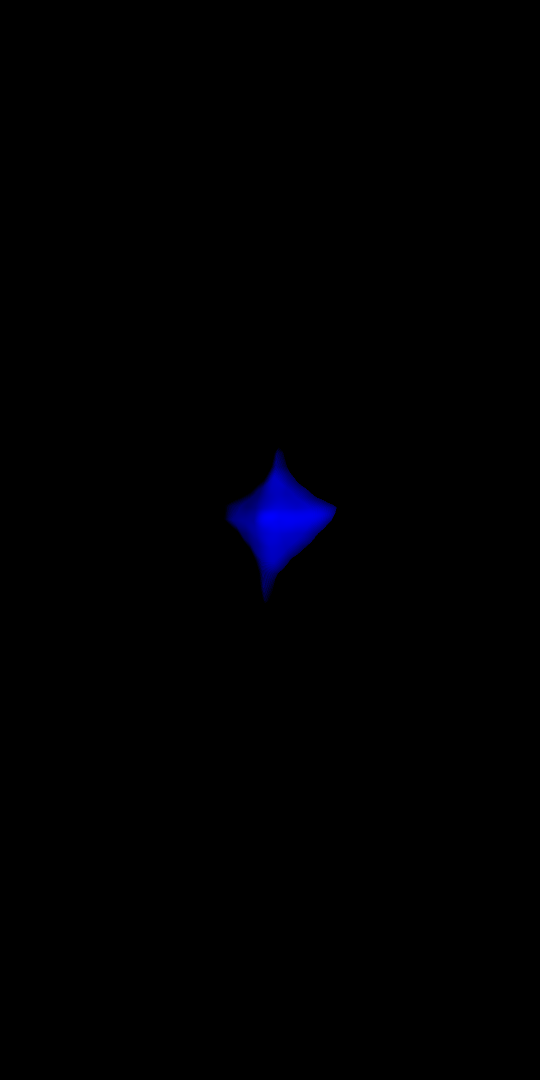
\includegraphics[width=.3\linewidth]{figures/bluecore/20.png}}
\caption
{
\label{fig:fire5}
A burning blue core visualized as a surface.
}
\end{figure}       

Link to a video which demonstrates all the results in the figures:
\href{http://youtu.be/F40\_rowaLQg}{Video link}


\section{Discussion}
Our implementation of the simulation and rendering achieves a detailed and visually plausable fire. Physically based variables can be fine tuned to achieve a wide variety of flame types by adjusting fuel injection speed, fuel ignition temperature, flame speed, fuel density, cooling constants etc.  Using world coordinates for our simulation grids enabled us to have different resolutions for different grids used in the simulation. For instance the temperature grid used for rendering can have considerably higher resolution than the grids used for the velocity fields in the same simulation run.

The design patterns used in our implementation is based on class inheritance, which turns out to be considerable performace hit, and created a sometimes unnecessary long simulation time. The current render method only samples from the simulation grids and does not perform any intersection tests against meshes or any triangles for that matter. We can therefore currently not render triangles, meshes, and so on or anything not present as data in the grids. The implemented calculation of the radiance values for the surrounding area is a quick method, but costly in memory since the radiance is calculated for every wavelength in every voxel, which is needed in order to calculate the mean radiance value. A more correct method would probable implement a Monte Carlo method instead.

\endgroup

\bibliographystyle{abbrv}
\bibliography{bibl}

\end{document}
